\documentclass[aspectratio=169,10pt]{beamer}
% =============================================================================
% PX4 + ROS 2 con px4_examples — Vespo UAV
%
% Compilar:  latexmk -pdf main.tex      (o pdflatex dos veces, por los índices)
% Necesita:  texlive-latex-extra texlive-lang-spanish texlive-pictures
%            texlive-fonts-recommended
%
% Cada sección vive en secciones/NN_nombre.tex. Todo lo que se cita del código
% sale de src/px4_examples/src/*.cpp.
% =============================================================================
% (el \documentclass va en cada presentación)

\usepackage[utf8]{inputenc}
\usepackage[T1]{fontenc}
\usepackage[spanish,es-nodecimaldot,es-noshorthands]{babel}
\usepackage{amsmath,amssymb}
\usepackage{booktabs}
\usepackage{graphicx}
\usepackage{xcolor}
\usepackage{listings}
\usepackage[most]{tcolorbox}
\usepackage{tikz}
\usetikzlibrary{arrows.meta,positioning,shapes.geometric,shapes.misc,calc,fit,backgrounds,decorations.pathreplacing}
\usepackage{multicol}
\usepackage{pifont}
% Lo que imprime vespo en la terminal
\DeclareUnicodeCharacter{2714}{\ding{51}}
\DeclareUnicodeCharacter{2718}{\ding{55}}
\DeclareUnicodeCharacter{2500}{\textendash}

\graphicspath{{img/}{img/px4docs/}{img/render/}{../../../x500_retos/docs/img/}}

% --- Tema: el de la intro a ROS2 ---------------------------------------------
\usetheme{default}
\useoutertheme{infolines}
\setbeamertemplate{headline}{}
\setbeamercolor{author in head/foot}{fg=black,bg=white}
\setbeamercolor{title in head/foot}{fg=blue!70!black,bg=white}
\setbeamercolor{date in head/foot}{fg=black,bg=white}
\setbeamercolor{section in toc}{fg=blue!70!black}
\setbeamertemplate{section in toc}[circle]
\setbeamercolor{frametitle}{fg=black,bg=white}
\setbeamerfont{frametitle}{size=\Large}
\setbeamertemplate{frametitle}{%
  \vskip0.4em
  \begin{beamercolorbox}[wd=\paperwidth,leftskip=0.3em,rightskip=0.3em]{frametitle}%
    \usebeamerfont{frametitle}\insertframetitle\hfill
    \raisebox{-0.45em}{
\includegraphics[height=1.6em]{vespo_logo}}%
  \end{beamercolorbox}}
\setbeamertemplate{caption}[numbered]
\setbeamertemplate{itemize items}[circle]
\setbeamercolor{itemize item}{fg=blue!70!black}
\setbeamercolor{enumerate item}{fg=blue!70!black}

% --- Colores y cajas -------------------------------------------------------------
\definecolor{azul}{RGB}{40,80,180}
\definecolor{azulclaro}{RGB}{232,238,252}
\definecolor{verde}{RGB}{0,128,0}
\definecolor{verdeclaro}{RGB}{236,250,236}
\definecolor{rojo}{RGB}{190,30,30}
\definecolor{naranja}{RGB}{230,120,10}
\definecolor{gris}{RGB}{110,110,110}

% Idea clave: caja azul redondeada con sombra.
\newtcolorbox{idea}[1][]{enhanced,colback=azulclaro,colframe=azul!40,arc=2mm,
  boxrule=0.4pt,drop shadow,left=1.5mm,right=1.5mm,top=1mm,bottom=1mm,#1}
% Ojo: lo que suele salir mal.
\newtcolorbox{ojo}[1][]{enhanced,colback=red!5,colframe=rojo!60,arc=2mm,boxrule=0.4pt,
  drop shadow,left=1.5mm,right=1.5mm,top=1mm,bottom=1mm,
  title={\small\bfseries Ojo},fonttitle=\small,coltitle=white,colbacktitle=rojo!80,#1}
% Salida de terminal: barra verde con el comando.
\newtcolorbox{terminal}[1]{enhanced,colback=verdeclaro,colframe=verde,arc=1mm,boxrule=0.6pt,
  title={\ttfamily\small #1},fonttitle=\ttfamily\small,coltitle=white,colbacktitle=verde,
  left=1mm,right=1mm,top=0.5mm,bottom=0.5mm,fontupper=\ttfamily\scriptsize}

% --- Código ----------------------------------------------------------------------
\renewcommand{\lstlistingname}{Código}
\lstset{
  basicstyle=\ttfamily\scriptsize,
  keywordstyle=\color{azul}\bfseries,
  commentstyle=\color{gris}\itshape,
  stringstyle=\color{verde},
  frame=single, rulecolor=\color{black},
  breaklines=true, columns=fullflexible, keepspaces=true,
  showstringspaces=false, captionpos=b, tabsize=2,
  xleftmargin=2pt, xrightmargin=2pt, aboveskip=4pt, belowskip=2pt,
  literate=
    {á}{{\'a}}1 {é}{{\'e}}1 {í}{{\'i}}1 {ó}{{\'o}}1 {ú}{{\'u}}1
    {Á}{{\'A}}1 {É}{{\'E}}1 {Í}{{\'I}}1 {Ó}{{\'O}}1 {Ú}{{\'U}}1
    {ñ}{{\~n}}1 {Ñ}{{\~N}}1 {ü}{{\"u}}1 {¿}{{?`}}1 {¡}{{!`}}1
    {°}{{$^\circ$}}1 {²}{{$^2$}}1 {·}{{$\cdot$}}1
    {→}{{$\rightarrow$}}2 {←}{{$\leftarrow$}}2 {≈}{{$\approx$}}1
    {▲}{{$\blacktriangle$}}1 {►}{{$\blacktriangleright$}}1 {│}{{|}}1 {─}{{-}}1
    {┌}{{+}}1 {┐}{{+}}1 {└}{{+}}1 {┘}{{+}}1 {├}{{+}}1 {┤}{{+}}1 {┼}{{+}}1
}
\lstdefinestyle{cpp}{language=C++,morekeywords={override,nullptr,constexpr,auto}}
\lstdefinestyle{bash}{language=bash,morekeywords={ros2,vespo,colcon}}
\lstdefinelanguage{yaml}{morecomment=[l]\#,morestring=[b]"}

% --- Atajos ---------------------------------------------------------------------
\newcommand{\cmd}[1]{\texttt{#1}}
\newcommand{\ok}{{\color{verde}\checkmark}}
\newcommand{\mal}{{\color{rojo}$\times$}}

% Al empezar cada sección: el contenido con la sección actual resaltada.
\AtBeginSection[]{%
  \begin{frame}{Contenido}
    \begin{multicols}{2}\scriptsize
      \tableofcontents[currentsection]
    \end{multicols}
  \end{frame}}

% Láminas que se arman paso a paso: en TikZ, "visible on=<3->" muestra un
% nodo desde el paso 3 y "alt=<2>{fill=...}{fill=...}" lo resalta en el paso 2.
\tikzset{
  invisible/.style={opacity=0,text opacity=0},
  visible on/.style={alt={#1{}{invisible}}},
  alt/.code args={<#1>#2#3}{\alt<#1>{\pgfkeysalso{#2}}{\pgfkeysalso{#3}}},
}
\newcommand{\credito}[1]{{\tiny\color{gris}#1}}

% El x500 recortado (tools/renders_x500.py + tools/recortar_iconos.py).
% \dronarriba{ancho}: visto desde arriba, la nariz hacia arriba de la imagen.
% Para girarlo a un yaw (0 = norte, positivo hacia el este) en TikZ: \node[rotate=-yaw].
\newcommand{\dronarriba}[1]{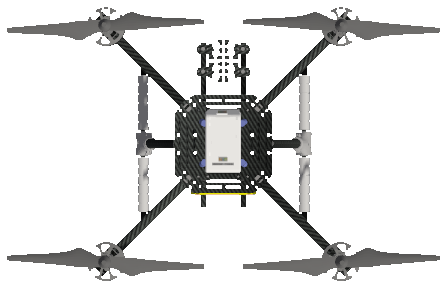
\includegraphics[width=#1]{x500_icono}}
\newcommand{\dronlado}[1]{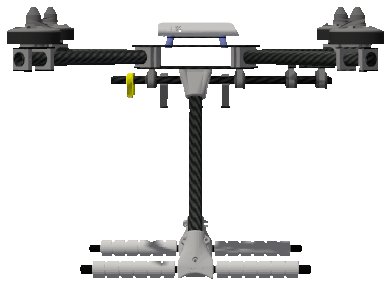
\includegraphics[width=#1]{x500_lado_icono}}


% --- Portada --------------------------------------------------------------------
\title[Referencia técnica]{PX4 + ROS 2 con px4\_examples: referencia técnica}
\subtitle{El x500, los mensajes de PX4 campo por campo y los 18 ejemplos con su código}
\author[Imad Cabrera]{Imad Jared Cabrera Trejo}
\institute[Vespo UAV]{Vespo UAV Drones Autónomos}
\date{11 de noviembre de 2026}

\begin{document}

\begin{frame}
  \titlepage
  \vspace{-1.5em}
  \begin{center}
\includegraphics[height=1.2cm]{vespo_logo}\end{center}
\end{frame}

\begin{frame}{Agenda}
  \begin{multicols}{2}\scriptsize
    \tableofcontents
  \end{multicols}
\end{frame}

% =============================================================================
\section{PX4 y el x500}
% =============================================================================

\begin{frame}{Idea central}
  \begin{columns}[c]
    \column{0.52\textwidth}
    \begin{idea}
      \textbf{PX4} es el piloto automático: el programa que corre en la controladora de vuelo y
      mantiene al dron en el aire. \textbf{ROS 2} es donde escribimos \emph{la misión}: qué hacer,
      a dónde ir, cuándo aterrizar.
    \end{idea}
    \vspace{0.4em}\small
    Nosotros \textbf{no controlamos los motores}: le pedimos cosas a PX4 (``ve a este punto'',
    ``aterriza'') y leemos lo que nos cuenta (posición, batería, modo).
    \column{0.45\textwidth}\centering
    \begin{tikzpicture}[node distance=0.5cm,every node/.style={font=\scriptsize},
        bx/.style={draw=azul,fill=azulclaro,rounded corners,minimum width=3.2cm,minimum height=0.7cm,align=center}]
      \node[bx,fill=yellow!20] (ros) {Tu nodo de ROS 2\\(la misión)};
      \node[bx,below=0.9cm of ros] (px4) {PX4\\(el piloto)};
      \node[bx,below=0.9cm of px4,fill=gray!15,draw=gray] (mot) {Motores y sensores};
      \draw[-{Stealth},thick] ([xshift=-0.6cm]ros.south) -- node[left]{pide} ([xshift=-0.6cm]px4.north);
      \draw[-{Stealth},thick] ([xshift=0.6cm]px4.north) -- node[right]{cuenta} ([xshift=0.6cm]ros.south);
      \draw[{Stealth}-{Stealth},thick] (px4) -- node[right]{400 Hz} (mot);
    \end{tikzpicture}
  \end{columns}
\end{frame}

\begin{frame}{¿Qué es PX4?}
  \begin{columns}[c]
  \column{0.68\textwidth}
  \begin{itemize}
    \item Un \textbf{autopiloto de código abierto} (BSD) para drones, aviones, VTOL, rovers y más.
    \item Corre en una \textbf{controladora de vuelo} (Pixhawk 6C, 6X, Cube\ldots) con un sistema
      operativo de tiempo real (NuttX).
    \item Por dentro son \textbf{módulos} independientes: sensores, estimador, controladores,
      \cmd{commander} (modos y armado), \cmd{navigator} (misiones), registro\ldots
    \item La misma base de código corre en \textbf{simulación} (SITL) en tu computadora.
    \item Usamos \textbf{PX4 v1.17.0} (fijado en \cmd{vespo.toml}); \cmd{px4\_msgs} tiene que coincidir.
  \end{itemize}
  \column{0.3\textwidth}\centering
  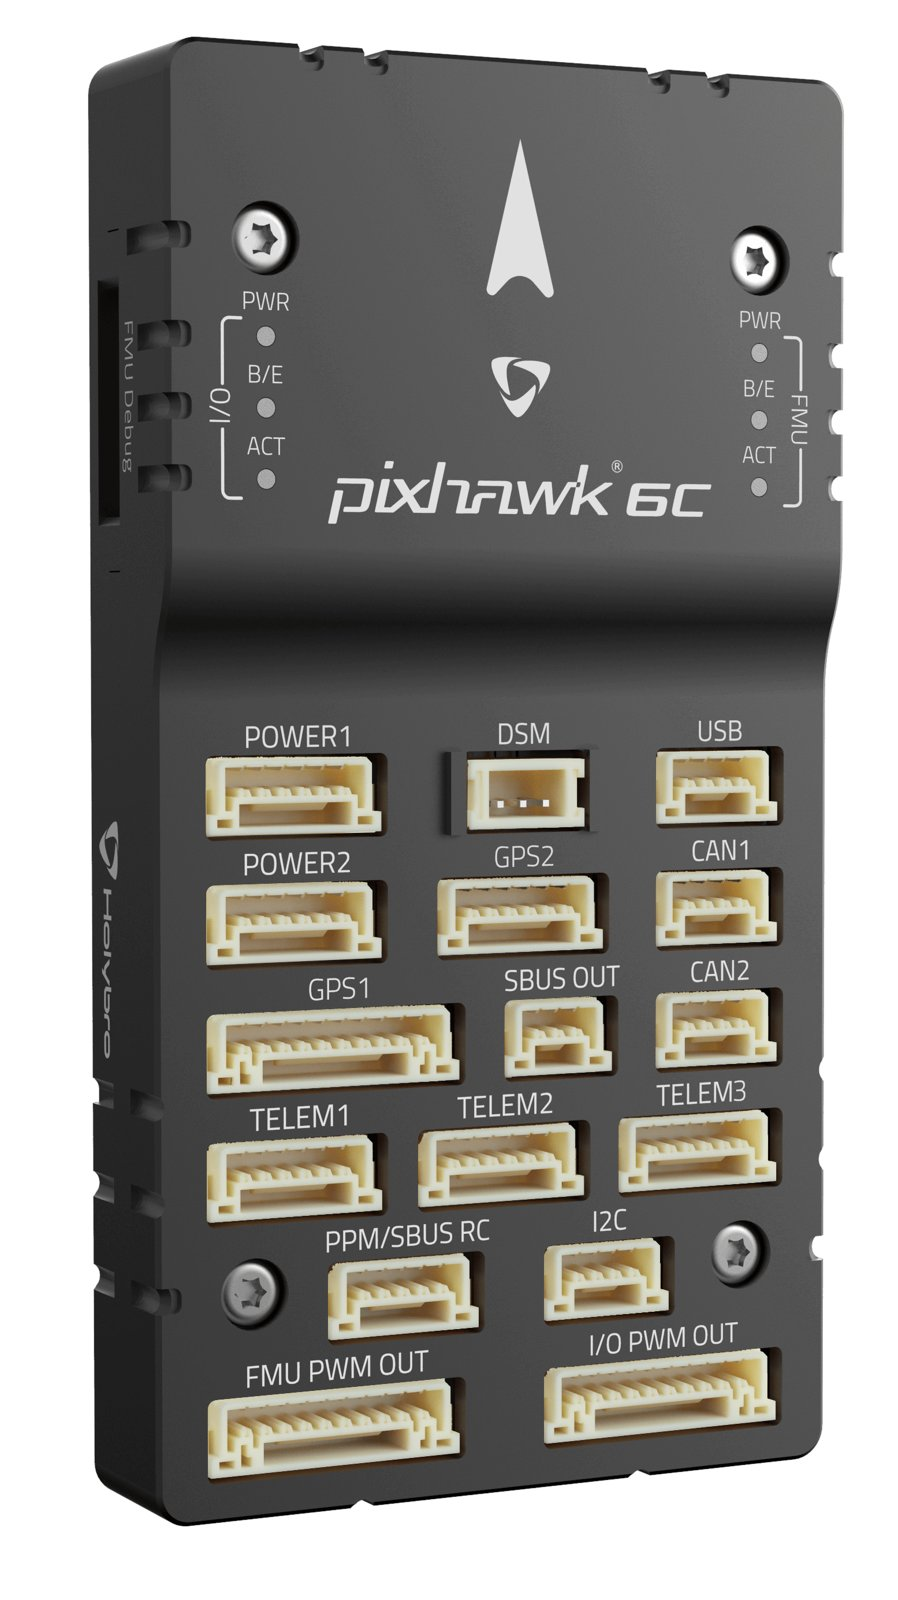
\includegraphics[height=0.55\textheight]{pixhawk6c}\\
  \credito{Pixhawk 6C. Docs de PX4 (CC BY 4.0)}
  \end{columns}
\end{frame}

\begin{frame}{Real contra simulación}
  \begin{columns}[t]
    \column{0.48\textwidth}\centering
    \textbf{En el dron}\\[0.4em]
    \begin{tikzpicture}[node distance=0.35cm,every node/.style={font=\tiny},
        bx/.style={draw=azul,fill=azulclaro,rounded corners,minimum width=2.6cm,align=center}]
      \node[bx] (c) {Computadora a bordo\\(Jetson / Raspberry Pi)\\ROS 2 + agente};
      \node[bx,below=of c] (p) {Pixhawk\\PX4};
      \node[bx,below=of p,fill=gray!15,draw=gray] (m) {ESC + motores, IMU, GPS};
      \draw[{Stealth}-{Stealth}] (c) -- node[right]{serial / USB} (p);
      \draw[{Stealth}-{Stealth}] (p) -- (m);
    \end{tikzpicture}
    \column{0.48\textwidth}\centering
    \textbf{En tu laptop (SITL)}\\[0.4em]
    \begin{tikzpicture}[node distance=0.35cm,every node/.style={font=\tiny},
        bx/.style={draw=azul,fill=azulclaro,rounded corners,minimum width=2.6cm,align=center}]
      \node[bx] (c) {ROS 2 + agente};
      \node[bx,below=of c] (p) {PX4 SITL\\(un proceso: bin/px4)};
      \node[bx,below=of p,fill=gray!15,draw=gray] (m) {Gazebo: física, motores\\y sensores simulados};
      \draw[{Stealth}-{Stealth}] (c) -- node[right]{UDP 8888} (p);
      \draw[{Stealth}-{Stealth}] (p) -- node[right]{gz\_bridge} (m);
    \end{tikzpicture}
  \end{columns}
  \vspace{0.4em}
  \begin{idea}
    \small Tu nodo \textbf{no sabe} si habla con un dron real o con la simulación: los topics son los mismos.
    Por eso todo se prueba primero en SITL.
  \end{idea}
\end{frame}

\begin{frame}{Por dentro: módulos que se hablan por uORB}
  \centering
  \begin{tikzpicture}[node distance=0.4cm,every node/.style={font=\tiny},
      md/.style={draw=azul,fill=azulclaro,rounded corners,minimum width=1.9cm,minimum height=0.55cm,align=center}]
    \node[md] (s) {sensores};
    \node[md,right=of s] (e) {EKF2\\(estimador)};
    \node[md,right=of e] (pc) {control de\\posición};
    \node[md,right=of pc] (ac) {control de\\actitud y rate};
    \node[md,right=of ac] (ca) {control\\allocation};
    \node[md,below=0.8cm of e] (cm) {commander\\(armado, modos)};
    \node[md,below=0.8cm of pc] (nv) {navigator\\(Takeoff, RTL\ldots)};
    \node[md,below=0.8cm of ac,fill=yellow!20] (dds) {uxrce\_dds\_client\\(puente a ROS 2)};
    \draw[-{Stealth}] (s) -- (e); \draw[-{Stealth}] (e) -- (pc); \draw[-{Stealth}] (pc) -- (ac); \draw[-{Stealth}] (ac) -- (ca);
    \draw[-{Stealth},dashed] (nv) -- (pc); \draw[-{Stealth},dashed] (cm) -- (nv);
    \draw[{Stealth}-{Stealth},dashed,naranja] (dds) -- (ac);
  \end{tikzpicture}
  \vspace{0.6em}
  \begin{itemize}\small
    \item \textbf{uORB}: el ``ROS interno'' de PX4. Cada módulo publica y se suscribe a \emph{topics} uORB
      (\cmd{vehicle\_local\_position}, \cmd{battery\_status}\ldots).
    \item El módulo \cmd{uxrce\_dds\_client} copia algunos de esos topics a ROS 2 y trae otros de vuelta.
  \end{itemize}
\end{frame}

\begin{frame}{El x500}
  \begin{columns}[c]
    \column{0.5\textwidth}\small
    \begin{itemize}
      \item Cuadricóptero de Holybro, marco en \textbf{X}, \textasciitilde500 mm de motor a motor en diagonal.
      \item Es el modelo por defecto de PX4 en Gazebo (\cmd{gz\_x500}, airframe \cmd{4001}).
      \item Variantes de PX4 con sensores: \cmd{x500\_lidar\_2d}, \cmd{x500\_mono\_cam\_down},
        \cmd{x500\_depth}\ldots
      \item En SITL flota (hover) con \textasciitilde60 \% de empuje (\cmd{MPC\_THR\_HOVER = 0.60}).
    \end{itemize}
    \column{0.47\textwidth}\centering
    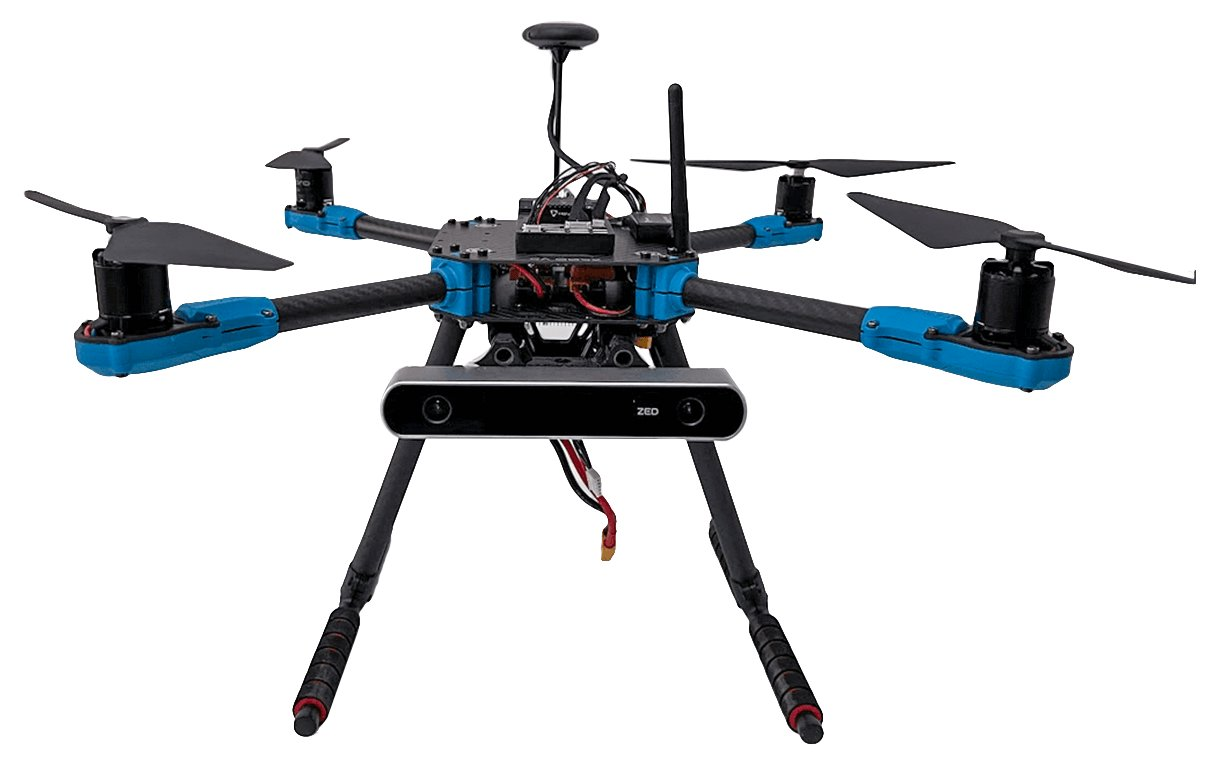
\includegraphics[width=\linewidth]{x500v2_armado}\\
    \credito{Holybro X500 V2. Documentación de PX4 (CC BY 4.0)}
  \end{columns}
\end{frame}

\begin{frame}{Los motores: número, posición y giro}
  \begin{columns}[c]
    \column{0.47\textwidth}\centering
    \begin{tikzpicture}[scale=1.25]
      \draw[line width=3pt,gray!60] (-1.1,1.1) -- (1.1,-1.1);
      \draw[line width=3pt,gray!60] (-1.1,-1.1) -- (1.1,1.1);
      \fill[gray!40] (-0.35,-0.35) rectangle (0.35,0.35);
      % motor 1: adelante derecha, CCW
      \draw[fill=azulclaro] (1.1,1.1) circle (0.42); \node[font=\small\bfseries] at (1.1,1.1) {1};
      \draw[-{Stealth},azul,thick] (1.1+0.55,1.1) arc (0:300:0.55);
      % motor 2: atrás izquierda, CCW
      \draw[fill=azulclaro] (-1.1,-1.1) circle (0.42); \node[font=\small\bfseries] at (-1.1,-1.1) {2};
      \draw[-{Stealth},azul,thick] (-1.1+0.55,-1.1) arc (0:300:0.55);
      % motor 3: adelante izquierda, CW
      \draw[fill=red!10] (-1.1,1.1) circle (0.42); \node[font=\small\bfseries] at (-1.1,1.1) {3};
      \draw[-{Stealth},rojo,thick] (-1.1+0.55,1.1) arc (0:-300:0.55);
      % motor 4: atrás derecha, CW
      \draw[fill=red!10] (1.1,-1.1) circle (0.42); \node[font=\small\bfseries] at (1.1,-1.1) {4};
      \draw[-{Stealth},rojo,thick] (1.1+0.55,-1.1) arc (0:-300:0.55);
      \draw[-{Stealth},thick,verde] (0,0) -- (0,0.9) node[above,font=\tiny] {x (frente)};
      \draw[-{Stealth},thick,rojo] (0,0) -- (0.9,0) node[right,font=\tiny,yshift=-6pt] {y (derecha)};
    \end{tikzpicture}
    \column{0.5\textwidth}\small
    Del airframe \cmd{4001\_gz\_x500} (en metros, marco FRD):
    \begin{center}\scriptsize
      \begin{tabular}{cccc}
        \toprule
        Motor & x & y & Giro \\
        \midrule
        1 & $+0.13$ & $+0.22$ & {\color{azul}antihorario} \\
        2 & $-0.13$ & $-0.20$ & {\color{azul}antihorario} \\
        3 & $+0.13$ & $-0.22$ & {\color{rojo}horario} \\
        4 & $-0.13$ & $+0.20$ & {\color{rojo}horario} \\
        \bottomrule
      \end{tabular}
    \end{center}
    \footnotesize Si en el dron real dos motores están cruzados, \textbf{se voltea al despegar}: para eso es
    \cmd{motor\_test}.
  \end{columns}
\end{frame}

\begin{frame}{Los motores en el x500 de la simulación}
  \begin{columns}[c]
    \column{0.5\textwidth}\centering
    \begin{tikzpicture}
      \node[anchor=south west,inner sep=0] (img) at (0,0) {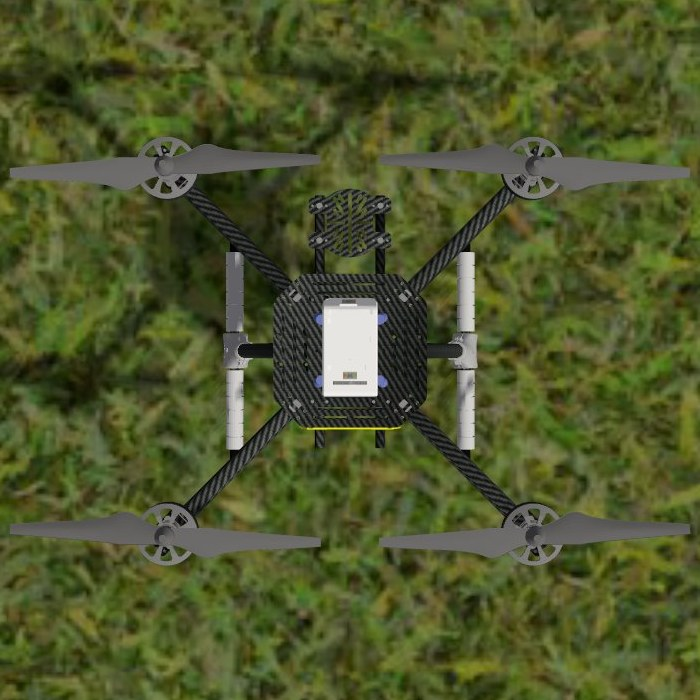
\includegraphics[height=0.72\textheight]{x500_arriba_recorte}};
      \begin{scope}[x={(img.south east)},y={(img.north west)}]
        \node[circle,fill=azul,text=white,font=\bfseries,inner sep=2.5pt] at (0.757,0.771) {1};
        \node[circle,fill=azul,text=white,font=\bfseries,inner sep=2.5pt] at (0.236,0.25) {2};
        \node[circle,fill=rojo,text=white,font=\bfseries,inner sep=2.5pt] at (0.236,0.771) {3};
        \node[circle,fill=rojo,text=white,font=\bfseries,inner sep=2.5pt] at (0.757,0.25) {4};
        \draw[-{Stealth},line width=2pt,verde] (0.5,0.62) -- (0.5,0.93);
        \node[font=\scriptsize\bfseries,verde,fill=white,inner sep=1pt] at (0.5,0.965) {FRENTE};
      \end{scope}
    \end{tikzpicture}\\
    \credito{Render propio de Gazebo, vista desde arriba}
    \column{0.47\textwidth}\centering
    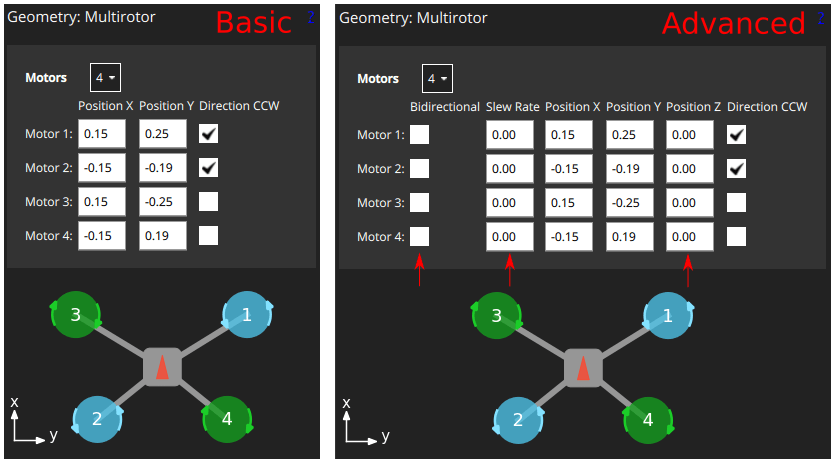
\includegraphics[width=\linewidth]{qgc_motores}\\
    \credito{QGroundControl. Docs de PX4 (CC BY 4.0)}\\[0.4em]
    \raggedright\small Mismo orden en el modelo de Gazebo, en el airframe y en QGC: {\color{azul}azul}
    antihorario, {\color{rojo}rojo} horario.
  \end{columns}
\end{frame}

\begin{frame}{¿Por qué la mitad gira al revés?}
  \begin{columns}[c]
    \column{0.55\textwidth}\small
    Cada hélice que gira empuja hacia arriba \textbf{y} tuerce el cuerpo en sentido contrario (par de
    reacción).
    \begin{itemize}
      \item Dos giran a un lado y dos al otro: los pares se \textbf{cancelan} y el dron no gira solo.
      \item Para \textbf{girar} (yaw), PX4 acelera un par y frena el otro: el empuje total es el mismo,
        pero los pares ya no se cancelan. Acelerar los antihorarios (1, 2) tuerce el cuerpo en sentido
        horario: yaw a la derecha.
    \end{itemize}
    \column{0.42\textwidth}
    \begin{idea}
      \small En el airframe esto es \cmd{CA\_ROTORn\_KM}: $+0.05$ gira antihorario, $-0.05$ horario. El
      \emph{control allocation} lo usa para repartir el giro.
    \end{idea}
  \end{columns}
\end{frame}

\begin{frame}{Cómo se mueve un cuadricóptero}
  \centering
  \begin{tikzpicture}[scale=0.55]
    \begin{scope}[shift={(0,0)}]
      \draw[line width=1.5pt,gray!60] (-1,1) -- (1,-1); \draw[line width=1.5pt,gray!60] (-1,-1) -- (1,1);
      \foreach \p in {(1,1),(-1,-1),(-1,1),(1,-1)} \fill[naranja] \p circle (0.38);
      \node[font=\tiny,align=center] at (0,-1.9) {\textbf{Subir}\\los 4 más rápido};
    \end{scope}
    \begin{scope}[shift={(4.5,0)}]
      \draw[line width=1.5pt,gray!60] (-1,1) -- (1,-1); \draw[line width=1.5pt,gray!60] (-1,-1) -- (1,1);
      \fill[naranja] (-1,1) circle (0.38); \fill[naranja] (-1,-1) circle (0.38);
      \fill[gray!40] (1,1) circle (0.38); \fill[gray!40] (1,-1) circle (0.38);
      \node[font=\tiny,align=center] at (0,-1.9) {\textbf{Roll} a la derecha\\izquierdos más rápido};
    \end{scope}
    \begin{scope}[shift={(9,0)}]
      \draw[line width=1.5pt,gray!60] (-1,1) -- (1,-1); \draw[line width=1.5pt,gray!60] (-1,-1) -- (1,1);
      \fill[naranja] (-1,-1) circle (0.38); \fill[naranja] (1,-1) circle (0.38);
      \fill[gray!40] (1,1) circle (0.38); \fill[gray!40] (-1,1) circle (0.38);
      \node[font=\tiny,align=center] at (0,-1.9) {\textbf{Pitch} adelante\\traseros más rápido};
    \end{scope}
    \begin{scope}[shift={(13.5,0)}]
      \draw[line width=1.5pt,gray!60] (-1,1) -- (1,-1); \draw[line width=1.5pt,gray!60] (-1,-1) -- (1,1);
      \fill[naranja] (1,1) circle (0.38); \fill[naranja] (-1,-1) circle (0.38);
      \fill[gray!40] (-1,1) circle (0.38); \fill[gray!40] (1,-1) circle (0.38);
      \node[font=\tiny,align=center] at (0,-1.9) {\textbf{Yaw} a la derecha\\los antihorarios (1, 2) más rápido};
    \end{scope}
  \end{tikzpicture}
  \vspace{0.4em}

  \raggedright\small Un multicóptero solo puede \textbf{inclinarse} y \textbf{empujar hacia ``arriba''} (de su cuerpo).
  Para avanzar se inclina: parte del empuje apunta hacia adelante.
\end{frame}

\begin{frame}{Los sensores}
  \centering\small
  \begin{tabular}{llll}
    \toprule
    Sensor & Mide & Frecuencia típica & Topic de ROS 2 \\
    \midrule
    Giroscopio & velocidad de giro (rad/s) & cientos de Hz & \cmd{/fmu/out/sensor\_combined} \\
    Acelerómetro & aceleración (m/s$^2$) & cientos de Hz & \cmd{/fmu/out/sensor\_combined} \\
    Barómetro & presión $\rightarrow$ altura & \textasciitilde50 Hz & (no expuesto) \\
    Magnetómetro & campo magnético $\rightarrow$ norte & \textasciitilde50 Hz & (no expuesto) \\
    GPS & latitud, longitud, altitud & 5--10 Hz & \cmd{/fmu/out/vehicle\_gps\_position} \\
    \bottomrule
  \end{tabular}
  \vspace{0.5em}
  \begin{idea}
    \small En SITL los \textbf{simula Gazebo} con ruido; PX4 los recibe por \cmd{gz\_bridge} como si fueran
    reales. Por eso el GPS de la simulación ``se mueve'' unos centímetros aunque el dron esté quieto.
  \end{idea}
\end{frame}

\begin{frame}{EKF2: de sensores a ``dónde estoy''}
  \begin{columns}[c]
    \column{0.5\textwidth}\centering
    \begin{tikzpicture}[node distance=0.25cm,every node/.style={font=\tiny},
        sn/.style={draw=gray,fill=gray!10,rounded corners,minimum width=1.6cm}]
      \node[sn] (i) {IMU};
      \node[sn,below=of i] (b) {barómetro};
      \node[sn,below=of b] (m) {magnetómetro};
      \node[sn,below=of m] (g) {GPS};
      \node[draw=azul,fill=azulclaro,rounded corners,minimum height=2.3cm,minimum width=1.4cm,right=1cm of b,yshift=-0.4cm] (e) {EKF2};
      \foreach \n in {i,b,m,g} \draw[-{Stealth}] (\n.east) -- (e.west);
      \node[draw=azul,rounded corners,right=0.7cm of e,align=left,font=\tiny] (o) {vehicle\_attitude\\vehicle\_local\_position\\vehicle\_global\_position};
      \draw[-{Stealth}] (e) -- (o);
    \end{tikzpicture}
    \column{0.47\textwidth}\small
    \begin{itemize}
      \item Un \textbf{filtro de Kalman extendido}: combina sensores que se equivocan de formas distintas.
      \item La IMU es rápida pero se desvía; el GPS es lento pero no se desvía: juntos dan una
        posición buena y rápida.
      \item Lo que leemos en ROS 2 (\cmd{vehicle\_local\_position}\ldots) es la \textbf{estimación}, no
        el sensor crudo.
    \end{itemize}
  \end{columns}
\end{frame}

\begin{frame}{La cadena de control (en cascada)}
  \centering
  \begin{tikzpicture}[node distance=0.3cm,every node/.style={font=\tiny},
      ct/.style={draw=azul,fill=azulclaro,rounded corners,minimum height=0.8cm,minimum width=1.55cm,align=center}]
    \node[ct] (p) {posición\\(P)};
    \node[ct,right=of p] (v) {velocidad\\(PID)};
    \node[ct,right=of v] (a) {aceleración\\$\rightarrow$ inclinación};
    \node[ct,right=of a] (at) {actitud\\(P)};
    \node[ct,right=of at] (r) {rate\\(PID)};
    \node[ct,right=of r] (c) {allocation\\$\rightarrow$ motores};
    \foreach \x/\y in {p/v,v/a,a/at,at/r,r/c} \draw[-{Stealth}] (\x) -- (\y);
    \node[below=0.15cm of p] {\textasciitilde50 Hz};
    \node[below=0.15cm of r] {\textasciitilde400+ Hz};
    \draw[decorate,decoration={brace,mirror,amplitude=4pt}] ([yshift=-0.7cm]p.south west) -- ([yshift=-0.7cm]a.south east) node[midway,below=4pt] {lo que mandamos en offboard};
  \end{tikzpicture}
  \vspace{0.6em}
  \begin{itemize}\small
    \item Cada lazo le da su \emph{setpoint} al siguiente: el de posición dice ``ve a 2 m/s'', el de velocidad
      dice ``inclínate 10°'', el de actitud dice ``gira a 1 rad/s''\ldots
    \item Los lazos de adentro son \textbf{más rápidos} que los de afuera.
    \item En offboard nosotros entramos \textbf{arriba}: posición, velocidad o aceleración.
  \end{itemize}
\end{frame}

\begin{frame}{Modos de vuelo (\texttt{nav\_state})}
  \centering\scriptsize
  \begin{tabular}{rll@{\hspace{1.2cm}}rll}
    \toprule
    \# & Modo & Quién manda & \# & Modo & Quién manda \\
    \midrule
    0 & Manual & piloto & 4 & Hold (Loiter) & PX4: quieto en un punto \\
    15 & Stabilized & piloto (nivela solo) & 17 & Takeoff & PX4: despega \\
    1 & Altitude & piloto, PX4 sostiene altura & 18 & Land & PX4: aterriza \\
    2 & Position & piloto, PX4 sostiene posición & 5 & Return (RTL) & PX4: a casa \\
    3 & Mission & PX4: plan de QGC & 21 & Orbit & PX4: círculo \\
    14 & \textbf{Offboard} & \textbf{tu nodo} & 12 & Descend & PX4: baja sin GPS \\
    \bottomrule
  \end{tabular}
  \vspace{0.6em}
  \raggedright\small
  \begin{itemize}
    \item En los ejemplos se compara con las constantes: \cmd{VehicleStatus::NAVIGATION\_STATE\_OFFBOARD}.
    \item \cmd{flight\_mode\_monitor} los imprime cada vez que cambian.
  \end{itemize}
\end{frame}

\begin{frame}{Dos maneras de mandar}
  \begin{columns}[t]
    \column{0.48\textwidth}
    \begin{idea}[title={\small\bfseries Offboard},coltitle=black,colbacktitle=azulclaro]
      \small Tu nodo calcula un \textbf{setpoint} 10--20 veces por segundo (posición, velocidad\ldots).
      \begin{itemize}
        \item Control fino: trayectorias, seguir algo.
        \item Si el nodo se cae, PX4 entra en \textbf{failsafe}.
        \item \cmd{takeoff\_mission}, \cmd{square\_mission}, \cmd{orbit\_mission}, \cmd{figure\_eight},
          \cmd{velocity\_control}.
      \end{itemize}
    \end{idea}
    \column{0.48\textwidth}
    \begin{idea}[title={\small\bfseries Comandos},coltitle=black,colbacktitle=azulclaro]
      \small Tu nodo manda \textbf{órdenes}: despega, ve a, orbita, regresa. PX4 vuela con sus modos.
      \begin{itemize}
        \item Menos código, más seguro: si el nodo se cae, PX4 sigue.
        \item Menos control fino.
        \item \cmd{orbit\_command}, \cmd{goto\_mission}, \cmd{return\_home}, \cmd{change\_speed},
          \cmd{set\_home}.
      \end{itemize}
    \end{idea}
  \end{columns}
\end{frame}

\begin{frame}{Armar}
  \begin{columns}[c]
    \column{0.55\textwidth}\small
    \textbf{Armar} = darle permiso a los motores de girar. Antes, PX4 corre los \textbf{preflight checks}:
    \begin{itemize}
      \item sensores calibrados y coherentes, EKF2 convergido,
      \item GPS con fix (si el modo lo necesita), batería suficiente,
      \item enlace con la estación de tierra (\cmd{NAV\_DLL\_ACT}),
      \item el modo pedido se puede usar ahora.
    \end{itemize}
    Si algo falla, rechaza el armado y lo dice en la consola y en QGC.
    \column{0.42\textwidth}
    \begin{terminal}{consola de PX4}
WARN Preflight Fail:\\
\ \ ekf2 missing data\\
WARN Preflight Fail:\\
\ \ No connection to the GCS\\
WARN Arming denied: Resolve\\
\ \ system health failures first
    \end{terminal}
    \small Al tocar tierra, PX4 \textbf{desarma solo} (unos segundos después).
  \end{columns}
\end{frame}

\begin{frame}{Failsafes}
  \small Cuando algo sale mal, PX4 toma el control y hace una acción configurada:
  \vspace{0.3em}
  \centering\scriptsize
  \begin{tabular}{lll}
    \toprule
    Situación & Parámetro & Acción típica \\
    \midrule
    Se dejan de recibir setpoints de offboard & \cmd{COM\_OF\_LOSS\_T}, \cmd{COM\_OBL\_RC\_ACT} & Hold / Return / Land \\
    Se pierde la estación de tierra & \cmd{NAV\_DLL\_ACT} & Return \\
    Batería baja / crítica & \cmd{BAT\_LOW\_THR}, \cmd{COM\_LOW\_BAT\_ACT} & aviso / Return / Land \\
    Se sale de la geocerca & \cmd{GF\_ACTION} & aviso / Hold / Return \\
    Se pierde el control remoto & \cmd{NAV\_RCL\_ACT} & Return \\
    \bottomrule
  \end{tabular}
  \vspace{0.4em}
  \raggedright
  \begin{idea}
    \small \cmd{/fmu/out/failsafe\_flags} trae una bandera por cada cosa que PX4 vigila; \cmd{flight\_mode\_monitor}
    las muestra.
  \end{idea}
\end{frame}

\begin{frame}[fragile]{Parámetros de PX4 (no son los de ROS)}
  \small PX4 tiene \textasciitilde1000 parámetros propios: ganancias, límites, alturas. Se ven y cambian en
  QGroundControl (Vehicle Setup $\rightarrow$ Parameters) o en la consola \cmd{pxh>}:
  \begin{lstlisting}[style=bash,caption={En la terminal donde corre PX4 SITL}]
pxh> param show MIS_TAKEOFF_ALT        # altura del modo Takeoff
pxh> param show MPC_XY_VEL_MAX         # velocidad horizontal máxima
pxh> param set RTL_RETURN_ALT 15       # altura a la que regresa Return
pxh> commander status                  # estado general
pxh> listener vehicle_local_position   # leer un topic uORB
  \end{lstlisting}
  \begin{ojo}
    \small No confundir con los parámetros de ROS 2 de nuestros nodos (\cmd{--ros-args -p radius:=8.0}):
    esos son de tu programa, no de PX4.
  \end{ojo}
\end{frame}

\begin{frame}{La simulación completa}
  \centering
  \begin{tikzpicture}[node distance=0.45cm,every node/.style={font=\tiny},
      bx/.style={draw=azul,fill=azulclaro,rounded corners,minimum height=0.8cm,minimum width=2cm,align=center}]
    \node[bx,fill=gray!15,draw=gray] (gz) {Gazebo Harmonic\\física, sensores};
    \node[bx,right=0.9cm of gz] (px) {PX4 SITL};
    \node[bx,right=0.9cm of px] (ag) {Agente\\Micro XRCE-DDS};
    \node[bx,right=0.9cm of ag,fill=yellow!20] (ros) {Tus nodos\\de ROS 2};
    \node[bx,below=0.8cm of px,fill=gray!15,draw=gray] (qgc) {QGroundControl};
    \draw[{Stealth}-{Stealth}] (gz) -- node[above]{gz\_bridge} (px);
    \draw[{Stealth}-{Stealth}] (px) -- node[above]{UDP 8888} (ag);
    \draw[{Stealth}-{Stealth}] (ag) -- node[above]{DDS} (ros);
    \draw[{Stealth}-{Stealth}] (px) -- node[right]{MAVLink (UDP 14550)} (qgc);
  \end{tikzpicture}
  \vspace{0.6em}
  \begin{itemize}\small
    \item \cmd{vespo up --sim} levanta todo esto: el agente, PX4 + Gazebo y QGroundControl.
    \item \textbf{Lockstep}: PX4 avanza al paso de Gazebo. Si la simulación va lenta, PX4 también; tu
      nodo (con el reloj de la pared) no.
  \end{itemize}
\end{frame}

% =============================================================================
\section{Cómo habla ROS 2 con PX4}
% =============================================================================

\begin{frame}{El puente: uXRCE-DDS}
  \centering
  \begin{tikzpicture}[node distance=0.4cm,every node/.style={font=\scriptsize},
      bx/.style={draw=azul,fill=azulclaro,rounded corners,minimum height=1cm,minimum width=2.4cm,align=center}]
    \node[bx] (u) {uORB\\(dentro de PX4)};
    \node[bx,right=0.6cm of u] (c) {uxrce\_dds\_client\\(módulo de PX4)};
    \node[bx,right=1.4cm of c] (a) {MicroXRCEAgent\\(en la computadora)};
    \node[bx,right=0.6cm of a,fill=yellow!20] (r) {topics de ROS 2\\/fmu/in, /fmu/out};
    \draw[{Stealth}-{Stealth}] (u) -- (c);
    \draw[{Stealth}-{Stealth},thick] (c) -- node[above]{XRCE} node[below,font=\tiny]{UDP o serial} (a);
    \draw[{Stealth}-{Stealth}] (a) -- node[above]{DDS} (r);
  \end{tikzpicture}
  \vspace{0.6em}
  \begin{itemize}\small
    \item DDS ``completo'' es pesado para una controladora: PX4 habla \textbf{XRCE-DDS}, la versión para
      microcontroladores.
    \item El \textbf{agente} traduce a DDS normal: del otro lado ROS 2 ve topics comunes y corrientes.
    \item Sin agente corriendo, \textbf{no hay ningún topic de PX4} en ROS 2.
    \item SITL: \cmd{MicroXRCEAgent udp4 -p 8888}. Dron real: por serial (\cmd{vespo up --real}).
  \end{itemize}
\end{frame}

\begin{frame}{El diagrama oficial}
  \centering
  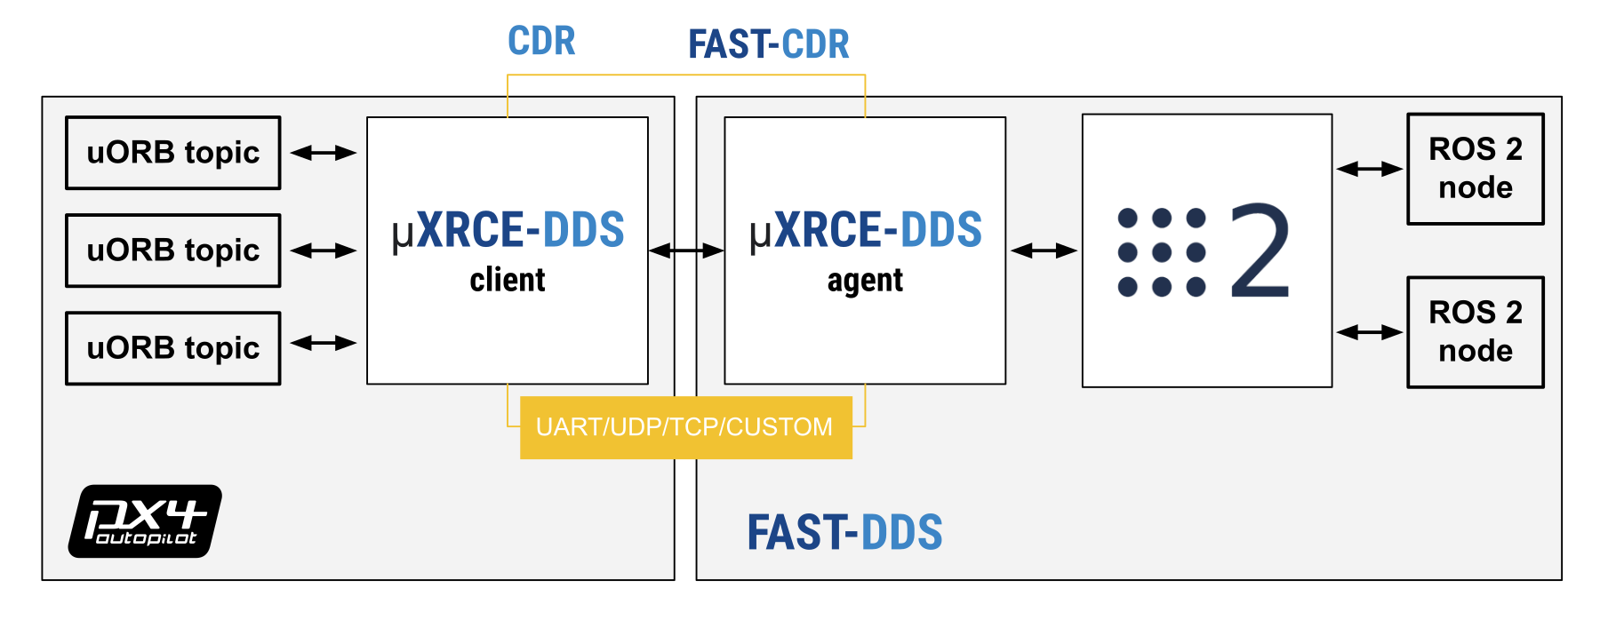
\includegraphics[width=0.95\linewidth]{xrce_dds}\\
  \credito{Arquitectura de uXRCE-DDS. Documentación de PX4 (CC BY 4.0)}
  \vspace{0.4em}

  \raggedright\small A la izquierda los topics uORB dentro de PX4; en medio el cliente (en PX4) y el agente (en la
  computadora) unidos por UART, UDP o TCP; a la derecha los nodos de ROS 2.
\end{frame}

\begin{frame}{/fmu/out y /fmu/in}
  \begin{columns}[t]
    \column{0.48\textwidth}
    \begin{idea}[title={\small\bfseries /fmu/out/\ldots: PX4 nos cuenta},coltitle=black,colbacktitle=azulclaro]
      \scriptsize
      \cmd{vehicle\_status\_v1}\\
      \cmd{vehicle\_local\_position\_v1}\\
      \cmd{vehicle\_global\_position}\\
      \cmd{vehicle\_attitude}\\
      \cmd{sensor\_combined}\\
      \cmd{vehicle\_gps\_position}\\
      \cmd{battery\_status\_v1}\\
      \cmd{home\_position\_v1}\\
      \cmd{failsafe\_flags}\\
      \cmd{vehicle\_command\_ack}
    \end{idea}
    \column{0.48\textwidth}
    \begin{idea}[title={\small\bfseries /fmu/in/\ldots: le pedimos a PX4},coltitle=black,colbacktitle=azulclaro]
      \scriptsize
      \cmd{offboard\_control\_mode}\\
      \cmd{trajectory\_setpoint}\\
      \cmd{vehicle\_command}
    \end{idea}
    \vspace{0.4em}\small
    Solo existen los topics que PX4 decide exponer: la lista está en
    \cmd{src/modules/uxrce\_dds\_client/dds\_topics.yaml} de PX4 (con su frecuencia máxima).
  \end{columns}
\end{frame}

\begin{frame}[fragile]{dds\_topics.yaml}
  \begin{lstlisting}[language=yaml,caption={Un pedazo del archivo de PX4 v1.17}]
publications:
  - topic: /fmu/out/battery_status
    type: px4_msgs::msg::BatteryStatus
    rate_limit: 1.            # a 1 Hz como mucho
  - topic: /fmu/out/vehicle_attitude
    type: px4_msgs::msg::VehicleAttitude
subscriptions:
  - topic: /fmu/in/trajectory_setpoint
    type: px4_msgs::msg::TrajectorySetpoint
  - topic: /fmu/in/vehicle_command
    type: px4_msgs::msg::VehicleCommand
  \end{lstlisting}
  \small Si un ejemplo no recibe nada, lo primero es revisar que el topic esté aquí y que el nombre sea
  exacto (incluido el sufijo de versión).
\end{frame}

\begin{frame}{Los sufijos \_v1: versiones de mensajes}
  \begin{columns}[c]
    \column{0.55\textwidth}\small
    Cuando PX4 cambia los campos de un mensaje, sube su \cmd{MESSAGE\_VERSION} y el topic cambia de nombre:
    \begin{center}\scriptsize
      \begin{tabular}{lcl}
        \toprule
        Mensaje & versión & topic \\
        \midrule
        \cmd{VehicleStatus} & 1 & \cmd{vehicle\_status\_v1} \\
        \cmd{VehicleLocalPosition} & 1 & \cmd{vehicle\_local\_position\_v1} \\
        \cmd{BatteryStatus} & 1 & \cmd{battery\_status\_v1} \\
        \cmd{HomePosition} & 1 & \cmd{home\_position\_v1} \\
        \cmd{VehicleGlobalPosition} & 0 & \cmd{vehicle\_global\_position} \\
        \cmd{VehicleAttitude} & 0 & \cmd{vehicle\_attitude} \\
        \bottomrule
      \end{tabular}
    \end{center}
    Versión 0 = sin sufijo.
    \column{0.42\textwidth}
    \begin{ojo}
      \small Si te suscribes a \cmd{/fmu/out/vehicle\_status} (sin \cmd{\_v1}) \textbf{no llega nada} y no hay
      ningún error: simplemente nadie publica en ese nombre.
    \end{ojo}
  \end{columns}
\end{frame}

\begin{frame}{px4\_msgs tiene que coincidir con PX4}
  \begin{columns}[c]
    \column{0.55\textwidth}\small
    \begin{itemize}
      \item \cmd{px4\_msgs} es un paquete de ROS 2 con los \textbf{mismos .msg} que tu versión de PX4.
      \item Si no coinciden, el agente no puede traducir: los topics ``existen'' pero los datos salen
        mal o no llegan.
      \item Por eso \cmd{vespo.toml} fija la versión de PX4 (v1.17.0) y \cmd{vespo.repos} el commit de
        \cmd{px4\_msgs} (\cmd{release/1.17}).
      \item \cmd{vespo px4 update} mueve los dos juntos.
    \end{itemize}
    \column{0.42\textwidth}\centering
    \begin{tikzpicture}[every node/.style={font=\tiny}]
      \node[draw=azul,fill=azulclaro,rounded corners,align=center] (p) {PX4 v1.17.0\\msg/*.msg};
      \node[draw=azul,fill=azulclaro,rounded corners,align=center,below=1cm of p] (m) {px4\_msgs\\release/1.17};
      \draw[{Stealth}-{Stealth},thick,verde] (p) -- node[right]{iguales} (m);
    \end{tikzpicture}
  \end{columns}
\end{frame}

\begin{frame}{QoS: cómo se entregan los mensajes}
  \small Cada publisher y subscriber de ROS 2 tiene una \textbf{calidad de servicio} (QoS). PX4 publica con:
  \begin{center}
    \cmd{rclcpp::QoS(1).best\_effort().transient\_local()}
  \end{center}
  \centering\scriptsize
  \begin{tabular}{lll}
    \toprule
    Parte & Significa & Por qué \\
    \midrule
    \cmd{QoS(1)} & guardar solo el último mensaje & solo importa el dato más reciente \\
    \cmd{best\_effort} & si se pierde uno, no se reenvía & a 100 Hz el siguiente llega enseguida \\
    \cmd{transient\_local} & al conectarte recibes el último que se publicó & no esperar al siguiente \\
    \bottomrule
  \end{tabular}
  \vspace{0.4em}
  \raggedright
  \begin{ojo}
    \small Un subscriber \cmd{reliable} \textbf{no recibe nada} de un publisher \cmd{best\_effort}. Por eso todos
    los ejemplos crean su suscripción con el mismo QoS que PX4.
  \end{ojo}
\end{frame}

\begin{frame}{Compatibilidad de QoS}
  \centering\small
  \begin{tabular}{llc}
    \toprule
    Publisher & Subscriber & ¿Se conectan? \\
    \midrule
    best\_effort & best\_effort & \ok \\
    reliable & best\_effort & \ok \\
    reliable & reliable & \ok \\
    best\_effort & reliable & \mal{} (nunca llega nada) \\
    \bottomrule
  \end{tabular}
  \vspace{0.6em}

  \raggedright\small
  \begin{itemize}
    \item Regla: el subscriber puede pedir \textbf{menos} que lo que ofrece el publisher, nunca más.
    \item Entre nodos nuestros (\cmd{battery\_publisher} $\rightarrow$ \cmd{battery\_subscriber}) usamos el
      QoS por defecto (reliable), porque no hace falta otra cosa.
    \item \cmd{ros2 topic info -v /fmu/out/vehicle\_status\_v1} muestra el QoS de cada lado.
  \end{itemize}
\end{frame}

\begin{frame}[fragile]{Timestamps: microsegundos desde que arrancó PX4}
  \small Todos los mensajes de PX4 empiezan con \cmd{uint64 timestamp}: tiempo desde que arrancó el sistema,
  en \textbf{microsegundos}.
  \begin{lstlisting}[style=cpp,caption={Así ponen el timestamp los ejemplos al publicar}]
uint64_t now_us() {
  return get_clock()->now().nanoseconds() / 1000;   // ns -> us
}
msg.timestamp = now_us();
  \end{lstlisting}
  \begin{itemize}
    \item Si un mensaje recibido tiene \cmd{timestamp == 0}, \textbf{todavía no ha llegado ninguno} (los
      mensajes nacen con todos sus campos en 0). \cmd{telemetry\_listener} lo usa para avisar.
    \item PX4 sincroniza su reloj con el del agente; en la práctica basta con mandar el tiempo actual.
  \end{itemize}
\end{frame}

\begin{frame}[fragile]{Explorar desde la terminal}
  \begin{lstlisting}[style=bash,caption={Con el agente y PX4 corriendo}]
ros2 topic list | grep fmu                            # qué expone PX4
ros2 topic echo /fmu/out/vehicle_status_v1 --once     # un mensaje
ros2 topic hz /fmu/out/sensor_combined                # qué tan rápido llega
ros2 interface show px4_msgs/msg/VehicleCommand       # los campos de un tipo
ros2 topic info -v /fmu/out/vehicle_local_position_v1 # QoS de cada lado
  \end{lstlisting}
  \begin{terminal}{ros2 topic echo /fmu/out/vehicle\_status\_v1 --field nav\_state}
14\\
---\\
14
  \end{terminal}
\end{frame}

% =============================================================================
\section{Los mensajes de PX4}
% =============================================================================

\begin{frame}[fragile]{Anatomía de un .msg}
  \begin{columns}[c]
    \column{0.52\textwidth}
    \begin{lstlisting}[language=yaml,caption={px4\_msgs/msg/VehicleCommandAck.msg (recortado)}]
uint32 MESSAGE_VERSION = 0       # constante

uint8 VEHICLE_CMD_RESULT_ACCEPTED = 0
uint8 VEHICLE_CMD_RESULT_DENIED = 2

uint64 timestamp      # campo: tipo nombre
uint32 command
uint8 result
    \end{lstlisting}
    \column{0.45\textwidth}\small
    \begin{itemize}
      \item Cada línea es \textbf{tipo nombre} (un campo) o \textbf{tipo NOMBRE = valor} (una constante).
      \item \cmd{colcon build} genera una \textbf{estructura de C++} con esos campos.
      \item Las constantes quedan como miembros estáticos:
        \cmd{VehicleCommandAck::VEHICLE\_CMD\_RESULT\_DENIED}.
    \end{itemize}
  \end{columns}
\end{frame}

\begin{frame}{Tipos de los .msg y su tipo en C++}
  \centering\small
  \begin{tabular}{lll}
    \toprule
    En el .msg & En C++ & Para qué \\
    \midrule
    \cmd{bool} & \cmd{bool} & banderas: \cmd{xy\_valid}, \cmd{failsafe} \\
    \cmd{uint8} & \cmd{uint8\_t} (0..255) & modos y estados: \cmd{nav\_state}, \cmd{arming\_state} \\
    \cmd{uint32} & \cmd{uint32\_t} & ids de comando: \cmd{command} \\
    \cmd{uint64} & \cmd{uint64\_t} & tiempos en µs: \cmd{timestamp} \\
    \cmd{float32} & \cmd{float} & casi todo: posición, velocidad, ángulos \\
    \cmd{float64} & \cmd{double} & latitud y longitud (necesitan precisión) \\
    \cmd{float32[3]} & \cmd{std::array<float, 3>} & vectores: \cmd{position}, \cmd{velocity} \\
    \cmd{float32[4]} & \cmd{std::array<float, 4>} & cuaterniones: \cmd{q} \\
    \bottomrule
  \end{tabular}
  \vspace{0.4em}

  \raggedright\footnotesize \cmd{float} tiene \textasciitilde7 dígitos: alcanza para metros, no para grados de latitud
  (47.3979711$^\circ$ necesita 9). Por eso \cmd{lat}/\cmd{lon} son \cmd{float64}.
\end{frame}

\begin{frame}[fragile]{Del .msg al \#include}
  \begin{lstlisting}[style=cpp,caption={El archivo va en snake\_case, el tipo en CamelCase}]
#include "px4_msgs/msg/vehicle_status.hpp"        // archivo: vehicle_status
using px4_msgs::msg::VehicleStatus;               // tipo: VehicleStatus

VehicleStatus status;                              // una variable de ese tipo
if (status.nav_state == VehicleStatus::NAVIGATION_STATE_OFFBOARD) { ... }
  \end{lstlisting}
  \small
  \begin{itemize}
    \item \cmd{px4\_msgs::msg::} es el \emph{namespace} (paquete \cmd{px4\_msgs}, carpeta \cmd{msg}).
    \item \cmd{using} evita escribir el nombre completo cada vez (como \cmd{from px4\_msgs.msg import ...} en Python).
  \end{itemize}
\end{frame}

\begin{frame}{VehicleStatus: el estado general}
  \begin{columns}[c]
    \column{0.55\textwidth}\centering\scriptsize
    \begin{tabular}{lll}
      \toprule
      Campo & Tipo & Qué es \\
      \midrule
      \cmd{arming\_state} & uint8 & 1 desarmado, 2 armado \\
      \cmd{nav\_state} & uint8 & el modo activo (14 = Offboard) \\
      \cmd{nav\_state\_user\_intention} & uint8 & el modo que \emph{pidió} el usuario \\
      \cmd{failsafe} & bool & ¿hay un failsafe activo? \\
      \cmd{pre\_flight\_checks\_pass} & bool & ¿se puede armar? \\
      \cmd{gcs\_connection\_lost} & bool & ¿se perdió QGC? \\
      \cmd{armed\_time} & uint64 & cuándo armó (µs) \\
      \bottomrule
    \end{tabular}
    \column{0.42\textwidth}\small
    Topic: \cmd{/fmu/out/vehicle\_status\_v1}.
    \vspace{0.3em}

    Es el \textbf{heartbeat} de PX4: casi todos los ejemplos lo leen para saber si ya armó y en qué modo
    está.
    \begin{idea}
      \small Si \cmd{nav\_state} $\neq$ \cmd{nav\_state\_user\_intention}, PX4 está haciendo otra cosa que lo
      que pediste (p. ej. un failsafe).
    \end{idea}
  \end{columns}
\end{frame}

\begin{frame}{VehicleLocalPosition: dónde estoy (en metros)}
  \begin{columns}[c]
    \column{0.55\textwidth}\centering\scriptsize
    \begin{tabular}{lll}
      \toprule
      Campo & Unidad & Qué es \\
      \midrule
      \cmd{x, y, z} & m & norte, este, abajo (NED) \\
      \cmd{vx, vy, vz} & m/s & velocidad NED \\
      \cmd{ax, ay, az} & m/s$^2$ & aceleración NED \\
      \cmd{heading} & rad & yaw, $-\pi..\pi$, 0 = norte \\
      \cmd{xy\_valid}, \cmd{z\_valid} & bool & ¿la estimación sirve? \\
      \cmd{dist\_bottom} & m & distancia al suelo (si hay sensor) \\
      \bottomrule
    \end{tabular}
    \column{0.42\textwidth}\small
    Topic: \cmd{/fmu/out/vehicle\_local\_position\_v1}.
    \begin{ojo}
      \small El origen es donde \textbf{arrancó PX4} (no donde está el dron ahora), y $z$ es hacia
      \textbf{abajo}: la altura es \cmd{-z}.
    \end{ojo}
  \end{columns}
\end{frame}

\begin{frame}{NED: el marco de VehicleLocalPosition}
  \begin{columns}[c]
    \column{0.45\textwidth}\centering
    \begin{tikzpicture}[scale=1.2]
      \draw[-{Stealth},thick,verde] (0,0) -- (0,1.8) node[above,font=\scriptsize] {x = Norte};
      \draw[-{Stealth},thick,rojo] (0,0) -- (1.8,0) node[right,font=\scriptsize] {y = Este};
      \draw[-{Stealth},thick,azul] (0,0) -- (0.9,-0.75) node[below right,font=\scriptsize] {z = Abajo};
      \fill (0,0) circle (1.5pt) node[below left,font=\tiny] {donde arrancó PX4};
      \fill[naranja] (0.8,1.2) circle (2.5pt) node[right,font=\tiny,black] {$(1.2,\ 0.8,\ -5)$: 5 m arriba};
    \end{tikzpicture}
    \column{0.52\textwidth}\small
    \begin{itemize}
      \item \textbf{N}orth, \textbf{E}ast, \textbf{D}own: el estándar de la aviación.
      \item Mandar $z = -5$ es pedir \textbf{5 m de altura}; $z = +5$ es pedir 5 m bajo tierra.
      \item ROS usa ENU (x este, y norte, z arriba). PX4 usa NED en todos sus mensajes: no hay que
        mezclarlos.
    \end{itemize}
  \end{columns}
\end{frame}

\begin{frame}{VehicleGlobalPosition: dónde estoy (en el planeta)}
  \begin{columns}[c]
    \column{0.55\textwidth}\centering\scriptsize
    \begin{tabular}{lll}
      \toprule
      Campo & Tipo & Qué es \\
      \midrule
      \cmd{lat}, \cmd{lon} & float64 & grados \\
      \cmd{alt} & float32 & m sobre el nivel del mar (AMSL) \\
      \cmd{lat\_lon\_valid}, \cmd{alt\_valid} & bool & ¿sirve? \\
      \cmd{eph}, \cmd{epv} & float32 & error estimado horiz./vert. (m) \\
      \bottomrule
    \end{tabular}
    \column{0.42\textwidth}\small
    Topic: \cmd{/fmu/out/vehicle\_global\_position}.
    \vspace{0.3em}

    Es la estimación del EKF2 (no el GPS crudo). Los comandos de PX4 (\cmd{NAV\_TAKEOFF},
    \cmd{DO\_REPOSITION}, \cmd{DO\_SET\_HOME}) piden coordenadas y \textbf{altitud AMSL}, no metros locales.
  \end{columns}
\end{frame}

\begin{frame}{VehicleAttitude: la orientación como cuaternión}
  \begin{columns}[c]
    \column{0.5\textwidth}\small
    Topic: \cmd{/fmu/out/vehicle\_attitude}. Un solo campo importante:
    \begin{center}\cmd{float32[4] q} \quad $= [w,\ x,\ y,\ z]$\end{center}
    la rotación del cuerpo (FRD) a NED.
    \begin{itemize}
      \item Un \textbf{cuaternión} describe una rotación con 4 números sin los problemas de los ángulos de
        Euler (\emph{gimbal lock}).
      \item Cuidado: PX4 lo da como $[w, x, y, z]$; ROS (\cmd{geometry\_msgs}) usa $[x, y, z, w]$.
    \end{itemize}
    \column{0.47\textwidth}\centering
    \begin{tikzpicture}[scale=1.0]
      \draw[thick,fill=gray!20,rotate=20] (-1,-0.12) rectangle (1,0.12);
      \draw[-{Stealth},verde,thick,rotate=20] (0,0) -- (1.5,0) node[right,font=\tiny] {frente};
      \draw[dashed,gray] (0,0) -- (1.6,0);
      \draw[-{Stealth},azul] (1.1,0) arc (0:20:1.1);
      \node[font=\tiny,azul] at (1.35,0.25) {pitch};
      \node[font=\tiny] at (0,-0.8) {roll, pitch, yaw = 3 ángulos};
      \node[font=\tiny] at (0,-1.1) {q = la misma rotación en 4 números};
    \end{tikzpicture}
  \end{columns}
\end{frame}

\begin{frame}[fragile]{De cuaternión a roll, pitch y yaw}
  \begin{lstlisting}[style=cpp,caption={telemetry\_listener.cpp}]
// PX4 da el cuaternión en orden [w, x, y, z] (ROS usa [x, y, z, w]).
const float w = attitude_.q[0];
const float x = attitude_.q[1];
const float y = attitude_.q[2];
const float z = attitude_.q[3];
const float roll = std::atan2(2.0f * (w * x + y * z), 1.0f - 2.0f * (x * x + y * y));
// asin solo acepta valores en [-1, 1]; std::clamp evita NaN por redondeo.
const float pitch = std::asin(std::clamp(2.0f * (w * y - z * x), -1.0f, 1.0f));
const float yaw = std::atan2(2.0f * (w * z + x * y), 1.0f - 2.0f * (y * y + z * z));
  \end{lstlisting}
  \small Con el dron nivelado: roll $\approx$ pitch $\approx 0$ y yaw = hacia dónde apunta la nariz (igual a
  \cmd{heading} de la posición local).
\end{frame}

\begin{frame}{SensorCombined: la IMU}
  \begin{columns}[c]
    \column{0.55\textwidth}\centering\scriptsize
    \begin{tabular}{lll}
      \toprule
      Campo & Unidad & Qué es \\
      \midrule
      \cmd{gyro\_rad[3]} & rad/s & velocidad de giro en x, y, z (FRD) \\
      \cmd{accelerometer\_m\_s2[3]} & m/s$^2$ & aceleración medida (FRD) \\
      \cmd{gyro\_integral\_dt} & µs & periodo de muestreo \\
      \cmd{accelerometer\_clipping} & bits & ¿se saturó algún eje? \\
      \bottomrule
    \end{tabular}
    \column{0.42\textwidth}\small
    Topic: \cmd{/fmu/out/sensor\_combined}, a cientos de Hz.
    \begin{idea}
      \small Quieto en el suelo el acelerómetro marca $(0, 0, -9.81)$: mide la fuerza que lo
      \textbf{sostiene} (el suelo empuja hacia arriba, que en FRD es $z$ negativa), no la gravedad.
    \end{idea}
  \end{columns}
\end{frame}

\begin{frame}{SensorGps: el GPS crudo}
  \small Topic: \cmd{/fmu/out/vehicle\_gps\_position} (versión 0: sin sufijo). Es lo que dice el receptor,
  \textbf{antes} del EKF2. Sirve para saber si ya se puede volar con GPS (\cmd{gps\_status}).
  \vspace{0.5em}

  \centering\scriptsize
  \begin{tabular}{ll}
    \toprule
    Campo & Qué es \\
    \midrule
    \cmd{fix\_type} & 0--1 sin fix, 2 = 2D, 3 = 3D, 4 = DGPS, 5 = RTK float, 6 = RTK fixed \\
    \cmd{satellites\_used} & satélites usados en la solución \\
    \cmd{eph}, \cmd{epv} & error estimado horizontal / vertical (m) \\
    \cmd{hdop} & qué tan buena es la geometría de los satélites ($<2$ es buena) \\
    \cmd{latitude\_deg}, \cmd{longitude\_deg} & posición (float64) \\
    \cmd{jamming\_state} & 0 desconocido, 1 OK, 2 mitigado, 3 interferencia detectada \\
    \bottomrule
  \end{tabular}
\end{frame}

\begin{frame}{BatteryStatus}
  \begin{columns}[c]
    \column{0.55\textwidth}\centering\scriptsize
    \begin{tabular}{lll}
      \toprule
      Campo & Unidad & Qué es (inválido) \\
      \midrule
      \cmd{connected} & bool & ¿hay batería? \\
      \cmd{voltage\_v} & V & voltaje total (0) \\
      \cmd{current\_a} & A & corriente ($-1$: sin sensor, como en SITL) \\
      \cmd{remaining} & 0..1 & carga restante ($-1$) \\
      \cmd{time\_remaining\_s} & s & hasta vacía (NaN) \\
      \cmd{cell\_count} & -- & celdas (4S = 4) \\
      \cmd{warning} & -- & 0 nada, 1 baja, 2 crítica, 3 emergencia \\
      \bottomrule
    \end{tabular}
    \column{0.42\textwidth}\small
    Topic: \cmd{/fmu/out/battery\_status\_v1}, a \textbf{1 Hz} (lo limita \cmd{dds\_topics.yaml}).
    \begin{ojo}
      \small Muchos campos usan un valor ``imposible'' para decir \textbf{no sé}: $-1$ o NaN. Revísenlo antes
      de usar el dato (\cmd{battery\_publisher} lo hace).
    \end{ojo}
  \end{columns}
\end{frame}

\begin{frame}{FailsafeFlags y HomePosition}
  \begin{columns}[t]
    \column{0.48\textwidth}\small
    \textbf{\cmd{/fmu/out/failsafe\_flags}}: \textasciitilde26 banderas (casi todas \cmd{bool}), una por cada cosa que PX4 vigila:
    \begin{itemize}\scriptsize
      \item \cmd{local\_position\_invalid}, \cmd{global\_position\_invalid}
      \item \cmd{home\_position\_invalid}
      \item \cmd{offboard\_control\_signal\_lost}
      \item \cmd{manual\_control\_signal\_lost}, \cmd{gcs\_connection\_lost}
      \item \cmd{battery\_warning}, \cmd{geofence\_breached}\ldots
    \end{itemize}
    \column{0.48\textwidth}\small
    \textbf{\cmd{/fmu/out/home\_position\_v1}}: ``casa'', a donde va Return.
    \begin{itemize}\scriptsize
      \item \cmd{lat}, \cmd{lon}, \cmd{alt}: en GPS
      \item \cmd{x}, \cmd{y}, \cmd{z}: en NED local
      \item \cmd{valid\_hpos}, \cmd{valid\_alt}
      \item \cmd{update\_count}: sube cada vez que casa cambia
    \end{itemize}
    PX4 la fija \textbf{donde arma} y solo la publica cuando cambia.
  \end{columns}
\end{frame}

\begin{frame}{VehicleCommand: pedirle algo a PX4}
  \begin{columns}[c]
    \column{0.55\textwidth}\centering\scriptsize
    \begin{tabular}{lll}
      \toprule
      Campo & Tipo & Qué es \\
      \midrule
      \cmd{command} & uint32 & qué comando (\cmd{VEHICLE\_CMD\_\ldots}) \\
      \cmd{param1..param4} & float32 & sus parámetros \\
      \cmd{param5, param6} & \textbf{float64} & normalmente lat, lon \\
      \cmd{param7} & float32 & normalmente altitud \\
      \cmd{target\_system} & uint8 & a quién va (1) \\
      \cmd{target\_component} & uint8 & 1 (0 = todos) \\
      \cmd{source\_system/component} & -- & quién lo manda (1, 1) \\
      \cmd{from\_external} & bool & \textbf{true}: viene de afuera de PX4 \\
      \bottomrule
    \end{tabular}
    \column{0.42\textwidth}\small
    Topic: \cmd{/fmu/in/vehicle\_command}.
    \vspace{0.3em}

    Son los comandos de \textbf{MAVLink} (los mismos que manda QGC): cada uno define qué significa cada
    parámetro.
  \end{columns}
\end{frame}

\begin{frame}{Los comandos que usan los ejemplos}
  \centering\scriptsize
  \begin{tabular}{lll}
    \toprule
    Comando & Parámetros & Ejemplos \\
    \midrule
    \cmd{DO\_SET\_MODE} & p1 = 1; p2 = 6 offboard, o p2 = 4 + p3 = 3 Hold & casi todos \\
    \cmd{COMPONENT\_ARM\_DISARM} & p1 = 1 armar, 0 desarmar & todos los que vuelan \\
    \cmd{NAV\_TAKEOFF} & p5, p6 = lat, lon; p7 = alt AMSL & orbit\_command, goto\ldots \\
    \cmd{NAV\_LAND} & --- & square, orbit, figure\_eight\ldots \\
    \cmd{NAV\_RETURN\_TO\_LAUNCH} & --- & orbit\_command, return\_home\ldots \\
    \cmd{DO\_REPOSITION} & p1 = vel, p2 = 1, p4 = yaw, p5..7 = lat, lon, alt & goto\_mission, change\_speed \\
    \cmd{DO\_ORBIT} & p1 = radio, p2 = vel, p5..7 = centro & orbit\_command \\
    \cmd{DO\_CHANGE\_SPEED} & p1 = 1 (suelo), p2 = m/s & change\_speed \\
    \cmd{DO\_SET\_HOME} & p1 = 0, p5..7 = lat, lon, alt & set\_home \\
    \cmd{ACTUATOR\_TEST} & p1 = 0..1, p2 = s, p5 = motor & motor\_test \\
    \bottomrule
  \end{tabular}
\end{frame}

\begin{frame}{VehicleCommandAck: ¿me hizo caso?}
  \begin{columns}[c]
    \column{0.5\textwidth}\centering\scriptsize
    \begin{tabular}{cl}
      \toprule
      \cmd{result} & Significa \\
      \midrule
      0 & ACCEPTED: aceptado y ejecutado \\
      1 & TEMPORARILY\_REJECTED: ahora no \\
      2 & DENIED: no, nunca \\
      3 & UNSUPPORTED: no lo conozco \\
      4 & FAILED: lo intenté y falló \\
      5 & IN\_PROGRESS: trabajando \\
      6 & CANCELLED \\
      \bottomrule
    \end{tabular}
    \column{0.47\textwidth}\small
    Topic: \cmd{/fmu/out/vehicle\_command\_ack}. Trae \cmd{command} (cuál) y \cmd{result}.
    \vspace{0.3em}
    \begin{terminal}{goto\_mission}
PX4 rechazó el comando 400\\
\ \ (result=1)
    \end{terminal}
    \footnotesize 400 = armar; 1 = ``ahora no'' (p. ej. falló un preflight check).
  \end{columns}
\end{frame}

\begin{frame}{OffboardControlMode: el heartbeat de offboard}
  \begin{columns}[c]
    \column{0.5\textwidth}\centering\scriptsize
    \begin{tabular}{ll}
      \toprule
      Campo (bool) & Controlar\ldots \\
      \midrule
      \cmd{position} & posición \\
      \cmd{velocity} & velocidad \\
      \cmd{acceleration} & aceleración \\
      \cmd{attitude} & actitud \\
      \cmd{body\_rate} & velocidad de giro \\
      \cmd{thrust\_and\_torque} & empuje y par \\
      \cmd{direct\_actuator} & los motores directo \\
      \bottomrule
    \end{tabular}
    \column{0.47\textwidth}\small
    Topic: \cmd{/fmu/in/offboard\_control\_mode}.
    \begin{itemize}
      \item Dice \textbf{qué tipo} de setpoint vamos a mandar.
      \item Hay que publicarlo \textbf{continuamente} (\textgreater2 Hz): si deja de llegar, PX4 sale de
        offboard (failsafe).
      \item Los ejemplos solo usan \cmd{position}, \cmd{velocity} y \cmd{acceleration}.
    \end{itemize}
  \end{columns}
\end{frame}

\begin{frame}{TrajectorySetpoint: a dónde ir}
  \begin{columns}[c]
    \column{0.5\textwidth}\centering\scriptsize
    \begin{tabular}{lll}
      \toprule
      Campo & Unidad & \\
      \midrule
      \cmd{position[3]} & m & NED \\
      \cmd{velocity[3]} & m/s & NED \\
      \cmd{acceleration[3]} & m/s$^2$ & NED \\
      \cmd{yaw} & rad & $-\pi..\pi$ \\
      \cmd{yawspeed} & rad/s & \\
      \bottomrule
    \end{tabular}
    \column{0.47\textwidth}\small
    Topic: \cmd{/fmu/in/trajectory\_setpoint}.
    \vspace{0.3em}

    \textbf{Lo que va en NaN, PX4 no lo usa}:
    \begin{itemize}
      \item posición + NaN en velocidad = ir al punto;
      \item NaN en posición + velocidad = ``joystick'' (\cmd{velocity\_control});
      \item yaw NaN + \cmd{yawspeed} = girar a cierta velocidad.
    \end{itemize}
  \end{columns}
\end{frame}

\begin{frame}[fragile]{NaN: ``no lo uses''}
  \begin{columns}[c]
    \column{0.55\textwidth}
    \begin{lstlisting}[style=cpp,caption={Como en goto\_mission y velocity\_control}]
#include <limits>
constexpr float kNaN = std::numeric_limits<float>::quiet_NaN();

msg.position = {kNaN, kNaN, kNaN};   // no controles posición
msg.velocity = {2.0f, 0.0f, 0.0f};   // 2 m/s al norte
msg.yaw = kNaN;                      // no fijes el yaw
    \end{lstlisting}
    \column{0.42\textwidth}\small
    \begin{itemize}
      \item NaN (\emph{Not a Number}) es un valor especial de \cmd{float}: el resultado de $0/0$.
      \item Cualquier comparación con NaN da \cmd{false}, \textbf{incluso} \cmd{x == x}.
      \item Para preguntar: \cmd{std::isnan(x)} o \cmd{std::isfinite(x)}.
    \end{itemize}
  \end{columns}
\end{frame}

\begin{frame}[fragile]{std\_msgs: mensajes que no son de PX4}
  \small Para pasarse un valor entre nodos nuestros no hace falta \cmd{px4\_msgs}:
  \begin{lstlisting}[language=yaml,caption={ros2 interface show std\_msgs/msg/Float32}]
float32 data
  \end{lstlisting}
  \begin{itemize}
    \item \cmd{battery\_publisher} publica el porcentaje de batería en \cmd{/vespo/battery\_percent} como
      \cmd{std\_msgs/Float32}.
    \item Cualquier nodo lo lee sin saber nada de PX4.
    \item Hay \cmd{Bool}, \cmd{Int32}, \cmd{String}, \cmd{Float64}\ldots y en \cmd{geometry\_msgs},
      \cmd{sensor\_msgs} mensajes más grandes (poses, imágenes, scans).
  \end{itemize}
\end{frame}

% =============================================================================
\section{Ejemplos de solo lectura}
% =============================================================================

\begin{frame}{Cinco nodos que solo escuchan}
  \centering\small
  \begin{tabular}{lll}
    \toprule
    Nodo & Lee & Para qué \\
    \midrule
    \cmd{telemetry\_listener} & estado, posición, GPS, actitud, batería & un resumen cada segundo \\
    \cmd{imu\_listener} & \cmd{sensor\_combined} & giroscopio y acelerómetro \\
    \cmd{gps\_status} & \cmd{vehicle\_gps\_position} & ¿ya se puede volar con GPS? \\
    \cmd{flight\_mode\_monitor} & \cmd{vehicle\_status\_v1}, \cmd{failsafe\_flags} & cada cambio de modo y failsafe \\
    \cmd{battery\_monitor} & \cmd{battery\_status\_v1} & avisar bajo un \% (y opcional RTL/LAND) \\
    \bottomrule
  \end{tabular}
  \vspace{0.6em}
  \begin{idea}
    \small No mandan nada a PX4 (salvo \cmd{battery\_monitor} si se lo piden): se pueden dejar corriendo
    \textbf{mientras} otro nodo vuela, para ver qué está pasando.
  \end{idea}
\end{frame}

\begin{frame}{El patrón: recibir en callbacks, imprimir en el timer}
  \centering
  \begin{tikzpicture}[node distance=0.35cm,every node/.style={font=\scriptsize},
      tp/.style={draw=gray,fill=gray!10,rounded corners,minimum width=3.2cm},
      mb/.style={draw=azul,fill=azulclaro,rounded corners,minimum width=1.8cm}]
    \node[tp] (t1) {vehicle\_status\_v1 (\textasciitilde5 Hz)};
    \node[tp,below=of t1] (t2) {vehicle\_local\_position (\textasciitilde50 Hz)};
    \node[tp,below=of t2] (t3) {vehicle\_attitude (\textasciitilde100 Hz)};
    \node[tp,below=of t3] (t4) {battery\_status\_v1 (1 Hz)};
    \node[mb,right=1.2cm of t1] (m1) {status\_};
    \node[mb,right=1.2cm of t2] (m2) {local\_};
    \node[mb,right=1.2cm of t3] (m3) {attitude\_};
    \node[mb,right=1.2cm of t4] (m4) {battery\_};
    \foreach \i in {1,2,3,4} \draw[-{Stealth}] (t\i) -- node[above,font=\tiny]{\cmd{= *msg}} (m\i);
    \node[draw=azul,fill=yellow!20,rounded corners,minimum height=2.6cm,right=1.2cm of m2,yshift=-0.45cm,align=center] (tm) {timer 1 s\\print\_summary()};
    \foreach \i in {1,2,3,4} \draw[-{Stealth},dashed] (m\i.east) -- (tm.west);
  \end{tikzpicture}
  \vspace{0.4em}

  \raggedright\small Cada topic llega a su ritmo; los callbacks solo guardan \textbf{la última copia}. El timer
  lee esas copias y escribe una sola línea por segundo, sin llenar la terminal.
\end{frame}

% ----------------------------------------------------------------------------- telemetry
\begin{frame}{telemetry\_listener}
  \begin{columns}[c]
    \column{0.5\textwidth}\small
    Se suscribe a 5 topics y cada segundo imprime:
    \begin{itemize}
      \item \textbf{Estado}: armado o no, y el modo (nombre y número).
      \item \textbf{Local}: x, y, altura ($-z$) y velocidad NED.
      \item \textbf{GPS}: lat, lon, alt (AMSL).
      \item \textbf{Actitud}: roll, pitch, yaw en grados (del cuaternión).
      \item \textbf{Batería}: voltaje y \%.
    \end{itemize}
    \column{0.47\textwidth}
    \begin{terminal}{ros2 run px4\_examples telemetry\_listener}
Estado: desarmado | modo: HOLD (4)\\
Local: x=0.01 y=-0.02 alt=0.03 m\\
\ \ | vel=(0.00, 0.00, 0.00) m/s\\
GPS: lat=47.3979711 lon=8.5461637\\
\ \ alt=0.1 m (AMSL)\\
Actitud: roll=0.1° pitch=-0.2° yaw=90.0°\\
Batería: 16.20 V | 100 \%
    \end{terminal}
  \end{columns}
\end{frame}

\begin{frame}[fragile]{telemetry\_listener: ¿llegaron datos?}
  \begin{lstlisting}[style=cpp,caption={telemetry\_listener.cpp}]
void print_summary() {
  // Si timestamp sigue en 0 es que todavía no ha llegado ningún mensaje
  // (los mensajes se crean con todos sus campos en 0). Suele indicar que
  // PX4 o el agente no están corriendo, o que el nombre del topic está mal.
  if (status_.timestamp == 0) {
    RCLCPP_WARN(get_logger(), "Sin datos de vehicle_status todavía (¿corre el agente?)");
    return;
  }
  ...
  \end{lstlisting}
  \small
  \begin{idea}
    \small Truco útil en cualquier nodo: un miembro con \cmd{timestamp == 0} significa ``nunca llegó un
    mensaje''. Antes de usar la posición, revisen que ya haya llegado (y que \cmd{xy\_valid} sea \cmd{true}).
  \end{idea}
\end{frame}

\begin{frame}[fragile]{telemetry\_listener: de \texttt{nav\_state} a texto}
  \begin{lstlisting}[style=cpp,caption={Una función que traduce el número a un nombre}]
const char * nav_state_name(uint8_t s) {
  switch (s) {
    case VehicleStatus::NAVIGATION_STATE_AUTO_LOITER: return "HOLD";
    case VehicleStatus::NAVIGATION_STATE_OFFBOARD:    return "OFFBOARD";
    case VehicleStatus::NAVIGATION_STATE_AUTO_LAND:   return "LAND";
    ...
    default: return "OTRO";   // cualquier otro valor
  }
}
  \end{lstlisting}
  \small \cmd{const char*} es texto fijo de C: lo que espera \cmd{\%s} en \cmd{RCLCPP\_INFO}. Cada \cmd{case}
  termina con \cmd{return}, así que no hace falta \cmd{break}.
\end{frame}

% ----------------------------------------------------------------------------- imu
\begin{frame}{imu\_listener}
  \begin{columns}[c]
    \column{0.5\textwidth}\small
    Lee \cmd{/fmu/out/sensor\_combined} (cientos de Hz) y muestra:
    \begin{itemize}
      \item \textbf{Gyro}: velocidad de giro en x, y, z (rad/s y °/s).
      \item \textbf{Accel}: aceleración en x, y, z (m/s$^2$).
      \item La frecuencia a la que llegan los mensajes.
    \end{itemize}
    Prueben girar el dron en Gazebo (o despegarlo con otro nodo) y vean cómo cambian.
    \column{0.47\textwidth}
    \begin{terminal}{ros2 run px4\_examples imu\_listener}
Gyro [rad/s]: x=+0.001 y=-0.002 z=+0.000\\
\ \ (deg/s: +0.1 -0.1 +0.0)\\
Accel [m/s²]: x=+0.012 y=-0.008\\
\ \ z=-9.806 | 250 Hz
    \end{terminal}
  \end{columns}
\end{frame}

\begin{frame}{¿Por qué el acelerómetro marca $-9.81$ quieto?}
  \begin{columns}[c]
    \column{0.45\textwidth}\centering
    \begin{tikzpicture}[scale=1]
      \fill[gray!30] (-1.6,-0.15) rectangle (1.6,0);
      \draw[thick,fill=azulclaro] (-0.6,0) rectangle (0.6,0.4);
      \draw[-{Stealth},thick,rojo] (0,0.2) -- (0,-1.1) node[below,font=\tiny] {gravedad};
      \draw[-{Stealth},thick,verde] (0.3,0.4) -- (0.3,1.5) node[above,font=\tiny] {el suelo empuja};
      \draw[-{Stealth},azul] (-1.1,0.2) -- (-1.1,-0.5) node[below,font=\tiny] {z (FRD)};
    \end{tikzpicture}
    \column{0.52\textwidth}\small
    \begin{itemize}
      \item Un acelerómetro mide la \textbf{fuerza específica}: todo menos la gravedad.
      \item Quieto en el suelo, lo único que siente es al suelo empujando \textbf{hacia arriba}.
      \item En FRD $z$ apunta hacia abajo, así que arriba es $z$ \textbf{negativa}: $(0, 0, -9.81)$.
      \item En caída libre marcaría $(0, 0, 0)$.
    \end{itemize}
  \end{columns}
\end{frame}

% ----------------------------------------------------------------------------- gps
\begin{frame}[fragile]{gps\_status}
  \begin{columns}[c]
    \column{0.5\textwidth}\small
    Lee el GPS \textbf{crudo} y dice si ya se puede volar con él. Revisa:
    \begin{itemize}
      \item \cmd{fix\_type} $\geq 3$ (3D),
      \item \cmd{satellites\_used} $\geq$ \cmd{min\_satellites} (6),
      \item \cmd{eph} $\leq$ \cmd{max\_eph} (3.0 m).
    \end{itemize}
    \begin{lstlisting}[style=bash]
ros2 run px4_examples gps_status --ros-args \
  -p min_satellites:=8 -p max_eph:=2.0
    \end{lstlisting}
    \column{0.47\textwidth}
    \begin{terminal}{ros2 run px4\_examples gps\_status}
3D | 10 sat | eph 0.9 m epv 1.4 m\\
\ \ | hdop 0.8 | 47.3979711, 8.5461637\\
\ \ GPS listo para volar
    \end{terminal}
    \footnotesize En el dron real, adentro de un edificio verán ``Todavía no:'' seguido de lo que falta.
  \end{columns}
\end{frame}

\begin{frame}{GPS crudo contra posición estimada}
  \centering
  \begin{tikzpicture}[node distance=0.5cm,every node/.style={font=\scriptsize},
      bx/.style={draw=azul,fill=azulclaro,rounded corners,minimum height=0.7cm,align=center}]
    \node[bx,fill=gray!15,draw=gray] (r) {receptor GPS};
    \node[bx,right=of r] (g) {\cmd{vehicle\_gps\_position}\\(crudo, 5--10 Hz)};
    \node[bx,right=of g] (e) {EKF2\\+ IMU, baro, mag};
    \node[bx,right=of e,fill=yellow!20] (o) {\cmd{vehicle\_global\_position}\\(estimado, rápido)};
    \draw[-{Stealth}] (r) -- (g); \draw[-{Stealth}] (g) -- (e); \draw[-{Stealth}] (e) -- (o);
    \node[below=0.2cm of g,font=\tiny] {\cmd{gps\_status}};
    \node[below=0.2cm of o,font=\tiny] {\cmd{telemetry\_listener}};
  \end{tikzpicture}
  \vspace{0.6em}

  \raggedright\small Para \textbf{volar} se usa la estimada; para \textbf{diagnosticar} el GPS (satélites,
  interferencia), la cruda.
\end{frame}

% ----------------------------------------------------------------------------- modos
\begin{frame}{flight\_mode\_monitor}
  \begin{columns}[c]
    \column{0.48\textwidth}\small
    Imprime \textbf{solo cuando algo cambia}:
    \begin{itemize}
      \item armado / desarmado,
      \item el modo (y si PX4 está en otro distinto del que pidió el usuario),
      \item failsafe activo / terminado,
      \item chequeos de pre-vuelo OK o fallando,
      \item las banderas de \cmd{failsafe\_flags} activas.
    \end{itemize}
    \column{0.5\textwidth}
    \begin{terminal}{ros2 run px4\_examples flight\_mode\_monitor}
DESARMADO\\
Modo: Hold\\
Chequeos de pre-vuelo: OK, se puede armar\\
ARMADO\\
Modo: Hold -> Offboard\\
Modo: Offboard -> Hold\\
FAILSAFE ACTIVO (modo Hold)\\
Banderas de failsafe:\\
\ \ señal offboard perdida
    \end{terminal}
  \end{columns}
\end{frame}

\begin{frame}[fragile]{flight\_mode\_monitor: comparar con lo anterior}
  \begin{lstlisting}[style=cpp,caption={flight\_mode\_monitor.cpp (recortado)}]
void on_status(const VehicleStatus & s) {
  if (first_ || s.nav_state != last_.nav_state) {
    RCLCPP_INFO(get_logger(), "Modo: %s -> %s", mode_name(last_.nav_state),
                mode_name(s.nav_state));
    // Si el modo activo no es el que pidió el usuario, PX4 lo cambió solo.
    if (s.nav_state != s.nav_state_user_intention) { ... }
  }
  last_ = s;          // guardar para la próxima comparación
  first_ = false;
}
  \end{lstlisting}
  \small Guardar el mensaje anterior y comparar es la forma de detectar \textbf{eventos} (cambios) en
  lugar de imprimir el estado una y otra vez.
\end{frame}

\begin{frame}{Úsenlo para entender qué hace PX4}
  \small Dejen \cmd{flight\_mode\_monitor} corriendo en una terminal y en otra:
  \begin{itemize}
    \item Corran \cmd{takeoff\_mission} y luego Ctrl+C: verán \textbf{Offboard $\rightarrow$ failsafe}.
    \item Corran \cmd{orbit\_command}: \textbf{Takeoff $\rightarrow$ Hold $\rightarrow$ Orbit $\rightarrow$
      Return $\rightarrow$ Land}.
    \item Cambien de modo desde QGroundControl.
  \end{itemize}
  \begin{idea}
    \small Cuando un nodo ``no hace nada'', casi siempre es porque PX4 está en un modo distinto del que
    creían. Este monitor lo dice en una línea.
  \end{idea}
\end{frame}

% ----------------------------------------------------------------------------- bateria
\begin{frame}{battery\_monitor}
  \begin{columns}[c]
    \column{0.5\textwidth}\small
    Lee la batería, avisa bajo \cmd{low\_percent} y, si se le pide, actúa:
    \begin{center}\scriptsize
      \begin{tabular}{ll}
        \toprule
        \cmd{action} & Qué hace \\
        \midrule
        \cmd{none} & solo avisa \\
        \cmd{rtl} & \cmd{NAV\_RETURN\_TO\_LAUNCH} \\
        \cmd{land} & \cmd{NAV\_LAND} ahí mismo \\
        \bottomrule
      \end{tabular}
    \end{center}
    Solo actúa si el dron \textbf{está armado}.
    \column{0.47\textwidth}
    \begin{terminal}{battery\_monitor -p low\_percent:=40.0 -p action:=rtl}
85.0 \% | 15.80 V (3.95 V/celda, 4S)\\
\ \ | -1.0 A | OK\\
BATERÍA BAJA: 39.8 \% (umbral 40 \%)\\
Regresando a casa (RTL)
    \end{terminal}
  \end{columns}
\end{frame}

\begin{frame}{El failsafe de PX4 contra el nuestro}
  \begin{columns}[c]
    \column{0.55\textwidth}\small
    PX4 ya tiene failsafe de batería (\cmd{BAT\_LOW\_THR}, \cmd{BAT\_CRIT\_THR}, \cmd{COM\_LOW\_BAT\_ACT}).
    ¿Para qué otro?
    \begin{itemize}
      \item Avisar \textbf{antes}, con un umbral propio de la misión.
      \item Que la \textbf{misión decida}: cortar, guardar dónde iba, ir a cargar (como la estación de
        carga del Nivel 3 de los retos).
    \end{itemize}
    \column{0.42\textwidth}
    \begin{ojo}
      \small En SITL \cmd{current\_a} es $-1$ (no hay sensor de corriente simulado) y la batería baja del 100 al
      50 \% en 30 s armado. No usen esos números para estimar el vuelo real.
    \end{ojo}
  \end{columns}
\end{frame}

% =============================================================================
\section{Un topic propio}
% =============================================================================

\begin{frame}{battery\_publisher y battery\_subscriber}
  \centering
  \begin{tikzpicture}[every node/.style={font=\scriptsize},
      bx/.style={draw=azul,fill=azulclaro,rounded corners,minimum height=0.8cm,minimum width=2.4cm,align=center}]
    \node[bx,fill=gray!15,draw=gray] (px) at (0,0) {PX4};
    \node[bx] (pub) at (4.4,0) {battery\_publisher\\(traduce)};
    \node[bx] (sub) at (9.4,0) {battery\_subscriber\\(muestra)};
    \node[bx,fill=gray!10,draw=gray] (any) at (9.4,-1.6) {cualquier otro nodo\\o \cmd{ros2 topic echo}};
    \draw[-{Stealth}] (px) -- node[above,font=\tiny,align=center]{battery\_status\_v1\\BatteryStatus} (pub);
    \draw[-{Stealth},thick,naranja] (pub) -- node[above,font=\tiny,align=center]{/vespo/battery\_percent\\std\_msgs/Float32} (sub);
    \draw[-{Stealth},thick,naranja] (pub.south) |- (any.west);
  \end{tikzpicture}
  \vspace{0.6em}
  \begin{itemize}\small
    \item Un nodo \textbf{traduce} lo que dice PX4 a algo simple: solo el porcentaje.
    \item Cualquier otro nodo lo usa \textbf{sin saber nada} de \cmd{px4\_msgs}: una interfaz, la misión, un
      registro\ldots
    \item Es el patrón para pasarse datos entre nodos nuestros.
  \end{itemize}
\end{frame}

\begin{frame}[fragile]{El publisher}
  \begin{lstlisting}[style=cpp,caption={battery\_publisher.cpp}]
// Publisher con QoS por defecto: rclcpp::QoS(10) = reliable, cola de 10.
percent_pub_ = create_publisher<Float32>("/vespo/battery_percent", 10);

auto px4_qos = rclcpp::QoS(1).best_effort().transient_local();
battery_sub_ = create_subscription<BatteryStatus>(
  "/fmu/out/battery_status_v1", px4_qos,
  [this](const BatteryStatus::SharedPtr msg) {
    // remaining = -1 cuando PX4 aún no sabe: no publicamos basura.
    if (!msg->connected || msg->remaining < 0.0f) {
      return;
    }
    Float32 out;
    out.data = msg->remaining * 100.0f;   // 0..1 -> 0..100 %
    percent_pub_->publish(out);
  });
  \end{lstlisting}
  \small Publica \textbf{dentro} del callback: cada vez que llega una batería de PX4 (1 Hz), sale un
  porcentaje. No hace falta timer.
\end{frame}

\begin{frame}{Las decisiones de diseño}
  \centering\small
  \begin{tabular}{lp{7.6cm}}
    \toprule
    Decisión & Por qué \\
    \midrule
    Nombre \cmd{/vespo/...} & Convención del equipo: nuestros topics no se confunden con los de PX4
      (\cmd{/fmu/...}) ni de otros paquetes. \\
    \cmd{std\_msgs/Float32} & Un mensaje estándar con un solo campo (\cmd{data}): no hace falta crear uno. \\
    QoS por defecto (\cmd{10}) & Entre nodos de ROS 2 no hace falta el best\_effort de PX4: reliable, cola de 10. \\
    Filtrar \cmd{remaining < 0} & $-1$ = ``PX4 no sabe'': mejor no publicar que publicar basura. \\
    \bottomrule
  \end{tabular}
\end{frame}

\begin{frame}[fragile]{El subscriber}
  \begin{lstlisting}[style=cpp,caption={battery\_subscriber.cpp}]
percent_sub_ = create_subscription<Float32>(
  "/vespo/battery_percent", 10,
  [this](const Float32::SharedPtr msg) {on_percent(msg->data);});

void on_percent(float percent) {
  // Barra de 20 caracteres: cada # vale 5 %.
  const int filled = static_cast<int>(percent / 5.0f + 0.5f);
  std::string bar;
  for (int i = 0; i < 20; i++) {
    bar += i < filled ? "#" : ".";
  }
  if (percent < low_percent_) {
    RCLCPP_WARN(get_logger(), "[%s] %5.1f %%  BAJA", bar.c_str(), percent);
  } else {
    RCLCPP_INFO(get_logger(), "[%s] %5.1f %%", bar.c_str(), percent);
  }
}
  \end{lstlisting}
\end{frame}

\begin{frame}{Detalles del subscriber}
  \begin{columns}[c]
    \column{0.52\textwidth}\small
    \begin{itemize}
      \item El callback llama a un método (\cmd{on\_percent}) con \textbf{solo el número}: el resto del código
        no sabe de mensajes.
      \item \cmd{+ 0.5f} antes de convertir a \cmd{int} \textbf{redondea} (sin él, \cmd{static\_cast} trunca:
        9.9 $\rightarrow$ 9).
      \item \cmd{bar.c\_str()}: \cmd{\%s} pide texto de C (\cmd{const char*}); \cmd{c\_str()} lo saca de un
        \cmd{std::string}.
    \end{itemize}
    \column{0.45\textwidth}
    \begin{terminal}{ros2 run px4\_examples battery\_subscriber}
[\#\#\#\#\#\#\#\#\#\#\#\#\#\#\#\#\#\#\#\#] 100.0 \%\\
[\#\#\#\#\#\#\#\#\#\#\#\#\#\#\#\#\#.\,.\,.] \ 84.5 \%\\
[\#\#\#\#\#.\,.\,.\,.\,.\,.\,.\,.\,.\,.\,.\,.\,.\,.\,.] \ 25.0 \%\ \ BAJA
    \end{terminal}
  \end{columns}
\end{frame}

\begin{frame}[fragile]{Probarlo sin PX4}
  \begin{lstlisting}[style=bash]
ros2 run px4_examples battery_subscriber            # terminal 1
ros2 topic pub /vespo/battery_percent std_msgs/msg/Float32 "{data: 15.0}"   # terminal 2
ros2 topic echo /vespo/battery_percent              # ver lo que pasa por el topic
ros2 topic info /vespo/battery_percent              # quién publica y quién escucha
  \end{lstlisting}
  \begin{idea}
    \small Como el subscriber solo depende del topic, se puede probar \textbf{sin simulación}: publiquen
    valores a mano para ver el aviso de batería baja. Así se prueban las partes de una misión por separado.
  \end{idea}
\end{frame}

\begin{frame}{Ejercicios}
  \begin{enumerate}\small
    \item Agreguen al publisher un segundo topic \cmd{/vespo/battery\_voltage} con el voltaje.
    \item Hagan que el subscriber avise \textbf{una sola vez} al cruzar el umbral (no en cada mensaje).
    \item Publiquen la altura actual (\cmd{-z} de \cmd{vehicle\_local\_position\_v1}) en
      \cmd{/vespo/altitude} y grafíquenla con \cmd{rqt\_plot}.
    \item Cambien el QoS del subscriber a \cmd{best\_effort}: ¿sigue funcionando? ¿Y si el que cambia es el
      publisher?
  \end{enumerate}
\end{frame}

% =============================================================================
\section{Offboard: nosotros calculamos}
% =============================================================================

\begin{frame}{Los cinco ejemplos de offboard}
  \centering\small
  \begin{tabular}{llll}
    \toprule
    Nodo & Qué vuela & Controla con & Lo nuevo \\
    \midrule
    \cmd{takeoff\_mission} & sube a 5 m y se queda & posición & el heartbeat \\
    \cmd{square\_mission} & cuadrado de 5 m y aterriza & posición & máquina de estados, waypoints \\
    \cmd{orbit\_mission} & círculo mirando al centro & posición + velocidad & parámetros, feedforward \\
    \cmd{figure\_eight} & un 8 en función del tiempo & + aceleración & derivadas, yaw de avance \\
    \cmd{velocity\_control} & tramos de velocidad & velocidad & NaN, marco del cuerpo \\
    \bottomrule
  \end{tabular}
  \vspace{0.6em}
  \begin{idea}
    \small Todos publican tres cosas: \cmd{OffboardControlMode} y \cmd{TrajectorySetpoint} \textbf{cada
    ciclo}, y \cmd{VehicleCommand} \textbf{una vez} para entrar a offboard y armar.
  \end{idea}
\end{frame}

\begin{frame}{El grafo de un nodo offboard}
  \centering
  \begin{tikzpicture}[node distance=0.4cm,every node/.style={font=\scriptsize},
      tp/.style={draw=gray,fill=gray!10,rounded corners,minimum width=3.6cm}]
    \node[draw=azul,fill=yellow!20,rounded corners,minimum height=3cm,minimum width=2.6cm] (n) {takeoff\_mission};
    \node[tp,left=1.2cm of n,yshift=0.6cm] (s) {/fmu/out/vehicle\_status\_v1};
    \node[tp,left=1.2cm of n,yshift=-0.6cm] (p) {/fmu/out/vehicle\_local\_position\_v1};
    \node[tp,right=1.2cm of n,yshift=0.9cm] (o) {/fmu/in/offboard\_control\_mode};
    \node[tp,right=1.2cm of n] (t) {/fmu/in/trajectory\_setpoint};
    \node[tp,right=1.2cm of n,yshift=-0.9cm] (c) {/fmu/in/vehicle\_command};
    \draw[-{Stealth}] (s) -- (n); \draw[-{Stealth}] (p) -- (n);
    \draw[-{Stealth}] (n) -- node[above,font=\tiny]{10 Hz} (o);
    \draw[-{Stealth}] (n) -- node[above,font=\tiny]{10 Hz} (t);
    \draw[-{Stealth}] (n) -- node[below,font=\tiny]{1 vez} (c);
  \end{tikzpicture}
\end{frame}

% ----------------------------------------------------------------------------- takeoff
\begin{frame}[fragile]{takeoff\_mission: el ciclo completo}
  \begin{lstlisting}[style=cpp,caption={takeoff\_mission.cpp, loop() a 10 Hz}]
// --- 1) Heartbeat: "sigo vivo y voy a controlar por POSICIÓN"
OffboardControlMode offboard_msg{};
offboard_msg.position = true;
offboard_msg.timestamp = now_us();
offboard_pub_->publish(offboard_msg);

// --- 2) Setpoint: z = -5 significa 5 m ARRIBA (NED)
TrajectorySetpoint setpoint_msg{};
setpoint_msg.position = {0.0f, 0.0f, -5.0f};
setpoint_msg.yaw = 0.0f;                // rad; 0 = mirando al norte
setpoint_msg.timestamp = now_us();
setpoint_pub_->publish(setpoint_msg);

// --- 3) Tras ~1 s de setpoints: pedir OFFBOARD y ARMAR (una sola vez)
if (counter_ == 10) {
  send_command(VehicleCommand::VEHICLE_CMD_DO_SET_MODE, 1.0f, 6.0f);     // 6 = OFFBOARD
  send_command(VehicleCommand::VEHICLE_CMD_COMPONENT_ARM_DISARM, 1.0f);  // 1 = armar
}
  \end{lstlisting}
\end{frame}

\begin{frame}{¿Por qué esperar 1 s antes de pedir offboard?}
  \centering
  \begin{tikzpicture}[x=1.05cm]
    \draw[-{Stealth}] (0,0) -- (11,0) node[right,font=\scriptsize] {ciclos (100 ms)};
    \foreach \x in {0,...,10} \draw[azul] (\x,0) -- (\x,0.3);
    \foreach \x in {0,...,10} \node[font=\tiny,below] at (\x,0) {\x};
    \node[font=\tiny,azul,above] at (5,0.35) {heartbeat + setpoint en cada ciclo};
    \draw[-{Stealth},thick,naranja] (10,1.2) -- (10,0.4);
    \node[font=\tiny,naranja,above,align=center] at (10,1.2) {counter\_ == 10:\\OFFBOARD + ARM};
  \end{tikzpicture}
  \vspace{0.6em}
  \begin{itemize}\small
    \item PX4 \textbf{rechaza} el cambio a offboard si no le están llegando setpoints \textbf{ya}: no sabría qué
      hacer en el primer instante.
    \item Por eso: primero \textasciitilde10 ciclos de setpoints, después los comandos.
    \item Y nunca se deja de publicar: si el nodo se cae (Ctrl+C), PX4 entra en \textbf{failsafe}
      (\cmd{COM\_OBL\_RC\_ACT}).
  \end{itemize}
\end{frame}

\begin{frame}[fragile]{send\_command(): el ayudante de todos}
  \begin{lstlisting}[style=cpp,caption={Igual en todos los ejemplos}]
void send_command(uint32_t command, float p1 = 0.0f, float p2 = 0.0f) {
  VehicleCommand msg{};
  msg.command = command;
  msg.param1 = p1;
  msg.param2 = p2;
  msg.target_system = 1;       // el dron (MAVLink system id)
  msg.target_component = 1;   // el autopiloto
  msg.source_system = 1;
  msg.source_component = 1;
  msg.from_external = true;    // viene de fuera de PX4 (de ROS 2)
  msg.timestamp = now_us();
  command_pub_->publish(msg);
}
  \end{lstlisting}
  \small \cmd{float p1 = 0.0f}: \textbf{valor por defecto}. \cmd{send\_command(VEHICLE\_CMD\_NAV\_LAND)} lo
  llama con \cmd{p1 = p2 = 0}.
\end{frame}

% ----------------------------------------------------------------------------- square
\begin{frame}[fragile]{square\_mission: waypoints y estados}
  \begin{columns}[c]
    \column{0.5\textwidth}
    \begin{lstlisting}[style=cpp]
enum class State { WARMUP, MISSION,
                   LANDING, DONE };

std::vector<std::array<float, 3>>
  waypoints_ = {
    {0.0f, 0.0f, -5.0f},   // WP0
    {5.0f, 0.0f, -5.0f},   // WP1
    {5.0f, 5.0f, -5.0f},   // WP2
    {0.0f, 5.0f, -5.0f},   // WP3
    {0.0f, 0.0f, -5.0f}};  // WP4
    \end{lstlisting}
    \column{0.47\textwidth}\centering
    \begin{tikzpicture}[scale=0.55]
      \draw[-{Stealth},verde] (0,0) -- (0,6.2) node[above,font=\tiny] {x (Norte)};
      \draw[-{Stealth},rojo] (0,0) -- (6.2,0) node[right,font=\tiny] {y (Este)};
      \draw[azul,thick,-{Stealth}] (0,0) -- (0,5) -- (5,5) -- (5,0) -- (0,0);
      \foreach \p/\n in {(0,0)/WP0,(0,5)/WP1,(5,5)/WP2,(5,0)/WP3} \fill[azul] \p circle (3pt) node[above left,font=\tiny] {\n};
    \end{tikzpicture}
  \end{columns}
  \small En MISSION manda el waypoint actual; cuando \cmd{reached()} da \cmd{true}, pasa al siguiente. Al
  terminar la lista: \cmd{NAV\_LAND}.
\end{frame}

\begin{frame}[fragile]{square\_mission: ¿ya llegué?}
  \begin{lstlisting}[style=cpp,caption={square\_mission.cpp}]
bool reached(const std::array<float, 3> & target) {
  float dx = position_.x - target[0];
  float dy = position_.y - target[1];
  float dz = position_.z - target[2];
  float distance = std::sqrt(dx*dx + dy*dy + dz*dz);
  return distance < 0.3f;
}
  \end{lstlisting}
  \begin{columns}[c]
    \column{0.55\textwidth}\small
    \begin{itemize}
      \item Distancia en 3D entre el dron y el waypoint.
      \item \textbf{0.3 m} de tolerancia: si es muy chica, el dron puede no ``llegar'' nunca por el ruido.
      \item En \cmd{LANDING} ya no publica setpoints: PX4 está en \cmd{AUTO\_LAND}.
    \end{itemize}
    \column{0.42\textwidth}
    \begin{terminal}{square\_mission}
Offboard activo, iniciando mision\\
Llegue al WP 0\\
Llegue al WP 1\\
\ldots\\
Mision completa, aterrizando
    \end{terminal}
  \end{columns}
\end{frame}

% ----------------------------------------------------------------------------- orbit
\begin{frame}{orbit\_mission: un círculo calculado por nosotros}
  \begin{columns}[c]
    \column{0.45\textwidth}\centering
    \begin{tikzpicture}[scale=0.9]
      \draw[gray] (0,0) circle (1.6);
      \fill (0,0) circle (2pt) node[below,font=\tiny] {centro};
      \fill[azul] (50:1.6) circle (3pt);
      \draw[-{Stealth},thick,naranja] (50:1.6) -- (50:0.5);
      \draw[-{Stealth},thick,azul] (50:1.6) -- ++(-40:0.9) node[right,font=\tiny] {$v$};
      \draw[-{Stealth},verde] (0,0) -- (0,2.2) node[above,font=\tiny] {N};
      \draw (0,0) -- (50:1.6) node[midway,above left,font=\tiny] {$r$};
      \draw[-{Stealth}] (0,0.6) arc (90:50:0.6);
      \node[font=\tiny] at (0.45,0.85) {$a$};
    \end{tikzpicture}
    \column{0.52\textwidth}\small
    \begin{itemize}
      \item Ángulo $a$ desde el norte, creciendo hacia el este (horario visto desde arriba).
      \item Punto: $(c_x + r\cos a,\ c_y + r\sin a)$.
      \item Cada ciclo: $a \mathrel{+}= \omega\,\Delta t$, con $\omega = v / r$ y $\Delta t = 0.1$ s.
      \item Velocidad (feedforward): $(-v\sin a,\ v\cos a)$, tangente al círculo.
      \item Yaw: mirando al centro.
    \end{itemize}
  \end{columns}
\end{frame}

\begin{frame}[fragile]{orbit\_mission: el estado ORBIT}
  \begin{lstlisting}[style=cpp,caption={orbit\_mission.cpp}]
case State::ORBIT: {
  // Las llaves {} crean un bloque: hacen falta para declarar variables
  // (omega) dentro de un case.
  const double omega = speed_ / radius_;
  // Derivada de (r cos a, r sin a): la velocidad es tangente al círculo.
  vx = -speed_ * std::sin(angle_);
  vy = speed_ * std::cos(angle_);
  angle_ += omega * kDt;

  if (angle_ >= 2.0 * M_PI * laps_) {
    send_command(VehicleCommand::VEHICLE_CMD_NAV_LAND);
    state_ = State::LANDING;
  }
  break;
}
  \end{lstlisting}
  \small \cmd{static constexpr double kDt = 0.1;}: el periodo del timer, como constante con nombre.
\end{frame}

\begin{frame}{Parámetros de orbit\_mission}
  \begin{columns}[c]
    \column{0.5\textwidth}\centering\small
    \begin{tabular}{llr}
      \toprule
      Parámetro & Qué & Defecto \\
      \midrule
      \cmd{center\_x} & m al norte & 0.0 \\
      \cmd{center\_y} & m al este & 0.0 \\
      \cmd{altitude} & m & 5.0 \\
      \cmd{radius} & m & 5.0 \\
      \cmd{speed} & m/s & 2.0 \\
      \cmd{laps} & vueltas (entero) & 2 \\
      \bottomrule
    \end{tabular}
    \column{0.47\textwidth}\small
    Pruébenlo con distintos valores \textbf{sin recompilar}:
    \begin{itemize}
      \item \cmd{-p radius:=8.0 -p speed:=3.0}
      \item \cmd{-p speed:=8.0}: ¿qué pasa con el error de seguimiento?
      \item \cmd{-p laps:=2.5}: \textbf{error}, \cmd{laps} es entero.
    \end{itemize}
  \end{columns}
\end{frame}

% ----------------------------------------------------------------------------- figure 8
\begin{frame}{figure\_eight: una curva en función del tiempo}
  \begin{columns}[c]
    \column{0.45\textwidth}\centering
    \begin{tikzpicture}[scale=0.9]
      \draw[azul,thick,domain=0:360,samples=120,smooth,variable=\t] plot ({0.75*sin(2*\t)}, {1.6*sin(\t)});
      \draw[-{Stealth},verde] (0,-1.9) -- (0,2) node[above,font=\tiny] {x (N)};
      \draw[-{Stealth},rojo] (-1.4,0) -- (1.4,0) node[right,font=\tiny] {y (E)};
      \fill (0,0) circle (2pt);
    \end{tikzpicture}
    \column{0.52\textwidth}\small
    La lemniscata de Gerono, con $w = 2\pi/T$:
    \[ x(t) = A\sin(wt) \qquad y(t) = \tfrac{A}{2}\sin(2wt) \]
    \begin{itemize}
      \item En $t = 0$ pasa por el origen: empieza donde despegó.
      \item $T$ (\cmd{period}) = segundos por cada 8; $A$ (\cmd{size}).
      \item Velocidad máxima $\approx A \cdot 2\pi / T$: con 5 m y 20 s, \textasciitilde1.6 m/s.
    \end{itemize}
  \end{columns}
\end{frame}

\begin{frame}{Derivar a mano: velocidad y aceleración}
  \small Con $\frac{d}{dt}\sin(wt) = w\cos(wt)$ y $\frac{d}{dt}\cos(wt) = -w\sin(wt)$:
  \[
    \begin{aligned}
      v_x &= A\,w\cos(wt) & v_y &= A\,w\cos(2wt) \\
      a_x &= -A\,w^2\sin(wt) & a_y &= -2A\,w^2\sin(2wt)
    \end{aligned}
  \]
  \begin{columns}[c]
    \column{0.55\textwidth}
    \begin{itemize}
      \item Se mandan \textbf{las tres}: posición, velocidad y aceleración.
      \item Sin feedforward, PX4 corrige \emph{después} de ver el error: se queda atrás de la curva.
      \item El nodo imprime el error de seguimiento: compárenlo quitando la velocidad.
    \end{itemize}
    \column{0.42\textwidth}
    \begin{idea}
      \small \textbf{Yaw de avance}: $\psi = \operatorname{atan2}(v_y, v_x)$. La nariz apunta hacia donde
      se mueve, como un coche.
    \end{idea}
  \end{columns}
\end{frame}

\begin{frame}[fragile]{figure\_eight: struct y método const}
  \begin{lstlisting}[style=cpp,caption={figure\_eight.cpp}]
// Posición, velocidad y aceleración de la curva en el instante t.
struct Sample { float x, y, vx, vy, ax, ay; };

Sample curve(double t) const {          // const: no cambia el objeto
  const double w = 2.0 * M_PI / period_;
  const double a = size_;
  return Sample{
    static_cast<float>(a * std::sin(w * t)),
    static_cast<float>(a / 2.0 * std::sin(2.0 * w * t)),
    ...
  };
}
  \end{lstlisting}
  \small
  \begin{itemize}
    \item \cmd{struct}: agrupar varios valores con nombre (como una clase con todo público).
    \item \cmd{const} después de los paréntesis: el método \textbf{promete} no modificar miembros.
    \item 20 Hz (timer de 50 ms): una trayectoria que cambia rápido se sigue mejor con más setpoints.
  \end{itemize}
\end{frame}

% ----------------------------------------------------------------------------- velocity
\begin{frame}{velocity\_control: como un joystick}
  \begin{columns}[c]
    \column{0.5\textwidth}\small
    Un plan de \textbf{tramos}: ``durante 4 s, 2 m/s al norte'', ``6 s girando a 0.5 rad/s''\ldots
    \begin{itemize}
      \item \cmd{OffboardControlMode}: \cmd{velocity = true}, \cmd{position = false}.
      \item Posición en \textbf{NaN}: ``no controles posición''.
      \item Yaw en NaN y \cmd{yawspeed} con valor: girar a cierta velocidad.
    \end{itemize}
    \column{0.47\textwidth}
    \begin{ojo}
      \small En velocidad el dron \textbf{no se queda en un punto}. Si mandas 0 se frena, pero con viento se
      va moviendo poco a poco: nadie corrige la posición.
    \end{ojo}
  \end{columns}
\end{frame}

\begin{frame}[fragile]{velocity\_control: el plan}
  \begin{lstlisting}[style=cpp,caption={velocity\_control.cpp: cambia, quita o agrega tramos}]
//   nombre                        fwd   right down  yawspeed  s    cuerpo
std::vector<Leg> legs_ = {
  {"norte a 2 m/s",                2.0f, 0.0f, 0.0f, 0.0f,    4.0, false},
  {"este a 2 m/s",                 0.0f, 2.0f, 0.0f, 0.0f,    4.0, false},
  {"girar en el lugar",            0.0f, 0.0f, 0.0f, 0.5f,    6.0, false},
  {"adelante (hacia donde mira)",  2.0f, 0.0f, 0.0f, 0.0f,    4.0, true},
  {"adelante girando (curva)",     2.0f, 0.0f, 0.0f, 0.4f,    6.0, true},
  {"bajar a 0.5 m/s",              0.0f, 0.0f, 0.5f, 0.0f,    3.0, false},
  {"frenar",                       0.0f, 0.0f, 0.0f, 0.0f,    2.0, false},
};
  \end{lstlisting}
  \small Un \cmd{std::vector} de \cmd{struct Leg}, inicializado con llaves. \cmd{cuerpo = true}: las
  velocidades son ``adelante / derecha'' del dron, no norte / este.
\end{frame}

\begin{frame}[fragile]{Del cuerpo a NED}
  \begin{lstlisting}[style=cpp,caption={velocity\_control.cpp}]
// Rotar (adelante, derecha) por el heading (yaw) del dron:
//   norte = adelante*cos(yaw) - derecha*sin(yaw)
//   este  = adelante*sin(yaw) + derecha*cos(yaw)
const float yaw = position_.heading;
vx = leg.forward * std::cos(yaw) - leg.right * std::sin(yaw);
vy = leg.forward * std::sin(yaw) + leg.right * std::cos(yaw);

setpoint_msg.position = {kNaN, kNaN, kNaN};   // si fuera {0,0,0}, ¡volvería al origen!
setpoint_msg.velocity = {vx, vy, leg.down};
setpoint_msg.yaw = kNaN;
setpoint_msg.yawspeed = leg.yawspeed;
  \end{lstlisting}
  \begin{columns}[c]
    \column{0.5\textwidth}\centering
    \begin{tikzpicture}[scale=0.8]
      \draw[-{Stealth},verde] (0,0) -- (0,1.8) node[above,font=\tiny] {N};
      \draw[-{Stealth},rojo] (0,0) -- (1.8,0) node[right,font=\tiny] {E};
      \draw[-{Stealth},thick,azul] (0,0) -- (40:1.6) node[above right,font=\tiny] {adelante};
      \draw[-{Stealth},thick,naranja] (0,0) -- (-50:1.2) node[right,font=\tiny] {derecha};
      \draw[-{Stealth}] (0,0.7) arc (90:40:0.7); \node[font=\tiny] at (0.4,0.95) {yaw};
    \end{tikzpicture}
    \column{0.47\textwidth}\small
    Es lo que se usa para \textbf{seguir algo con la cámara}: ``avanza hacia donde miras''.
  \end{columns}
\end{frame}

\begin{frame}{El despegue se cierra con la altura, no con el tiempo}
  \begin{columns}[c]
    \column{0.55\textwidth}\small
    Tentación: ``sube 5 s a 1 m/s'' = 5 m. En la práctica \textbf{no}:
    \begin{itemize}
      \item PX4 tarda en arrancar motores y hace una rampa de despegue.
      \item Con el tiempo como criterio, el dron se queda casi en el suelo cuando empieza el siguiente tramo.
    \end{itemize}
    \cmd{velocity\_control} sube a 1 m/s \textbf{hasta medir} la altura objetivo; luego empiezan los tramos.
    \column{0.42\textwidth}
    \begin{idea}
      \small Regla general: las transiciones de una misión se disparan con \textbf{lo que se mide} (posición,
      altura, modo), no con lo que \emph{debería} haber pasado.
    \end{idea}
  \end{columns}
\end{frame}

\begin{frame}{Seguridad en offboard: soltar el control}
  \begin{columns}[c]
    \column{0.55\textwidth}\small
    Todos los ejemplos de offboard revisan en cada ciclo:
    \begin{center}
      \cmd{state\_ != WARMUP \&\& !in\_offboard()} $\Rightarrow$ abortar
    \end{center}
    \begin{itemize}
      \item Si el piloto cambia de modo desde QGC o el control remoto, o hay un failsafe, el nodo
        \textbf{deja de mandar} y termina.
      \item Así el nodo nunca ``pelea'' contra el piloto.
    \end{itemize}
    \column{0.42\textwidth}
    \begin{terminal}{orbit\_mission}
Fuera de OFFBOARD (nav=4):\\
\ \ misión abortada
    \end{terminal}
  \end{columns}
\end{frame}

% =============================================================================
\section{Comandos: PX4 vuela}
% =============================================================================

\begin{frame}{Los seis ejemplos con comandos}
  \centering\small
  \begin{tabular}{lll}
    \toprule
    Nodo & Qué hace & Comandos \\
    \midrule
    \cmd{orbit\_command} & despega, orbita, regresa & TAKEOFF, DO\_ORBIT, RETURN \\
    \cmd{goto\_mission} & el cuadrado por coordenadas GPS & TAKEOFF, DO\_REPOSITION, RETURN \\
    \cmd{return\_home} & se aleja y muestra las fases de Return & TAKEOFF, DO\_REPOSITION, RETURN \\
    \cmd{change\_speed} & cambia la velocidad en pleno vuelo & DO\_REPOSITION, DO\_CHANGE\_SPEED \\
    \cmd{set\_home} & mueve ``casa'' y aterriza ahí & DO\_SET\_HOME, RETURN \\
    \cmd{motor\_test} & gira un motor, desarmado & ACTUATOR\_TEST \\
    \bottomrule
  \end{tabular}
  \vspace{0.6em}
  \begin{idea}
    \small Sin heartbeat ni setpoints: el nodo manda \textbf{una orden} y espera a que PX4 la cumpla
    (mirando el modo, la posición o el ack). Si el nodo se cae, PX4 sigue en su modo.
  \end{idea}
\end{frame}

\begin{frame}{El patrón: mandar, esperar, mandar}
  \centering
  \begin{tikzpicture}[node distance=0.35cm,every node/.style={font=\tiny},
      st/.style={draw=azul,fill=azulclaro,rounded corners,minimum width=1.9cm,minimum height=0.55cm,align=center}]
    \node[st] (g) {WAIT\_GPS};
    \node[st,right=of g] (a) {ARMING};
    \node[st,right=of a] (t) {TAKEOFF};
    \node[st,right=of t,fill=yellow!20] (m) {la acción\\(GOTO, ORBIT\ldots)};
    \node[st,right=of m] (r) {RETURN};
    \node[st,right=of r] (d) {DONE};
    \draw[-{Stealth}] (g) -- node[above]{GPS ok} (a);
    \draw[-{Stealth}] (a) -- node[above]{armó} (t);
    \draw[-{Stealth}] (t) -- node[above,align=center]{Hold y\\a la altura} (m);
    \draw[-{Stealth}] (m) -- node[above]{terminó} (r);
    \draw[-{Stealth}] (r) -- node[above]{desarmó} (d);
  \end{tikzpicture}
  \vspace{0.6em}
  \begin{itemize}\small
    \item Cada estado manda su comando \textbf{una vez} al entrar y luego \textbf{solo mira}.
    \item ``Terminó'' se mide: el modo cambió a Hold, la distancia al punto es pequeña, desarmó\ldots
  \end{itemize}
\end{frame}

\begin{frame}[fragile]{send\_command con los 7 parámetros}
  \begin{lstlisting}[style=cpp,caption={goto\_mission.cpp: param5 y param6 son double}]
void send_command(uint32_t command, float p1 = 0.0f, float p2 = 0.0f, float p3 = 0.0f,
  float p4 = 0.0f, double p5 = 0.0, double p6 = 0.0, float p7 = 0.0f)
{
  VehicleCommand msg{};
  msg.command = command;
  msg.param1 = p1;  msg.param2 = p2;  msg.param3 = p3;  msg.param4 = p4;
  msg.param5 = p5;  msg.param6 = p6;  msg.param7 = p7;
  ...
  command_pub_->publish(msg);
}
  \end{lstlisting}
  \small En MAVLink, param5 y param6 suelen ser latitud y longitud: en \cmd{float} se perdería
  \textasciitilde1 m. Por eso en \cmd{VehicleCommand} son \cmd{float64}.
\end{frame}

\begin{frame}[fragile]{Leer el ack: ¿por qué no me hizo caso?}
  \begin{lstlisting}[style=cpp,caption={goto\_mission.cpp}]
ack_sub_ = create_subscription<VehicleCommandAck>(
  "/fmu/out/vehicle_command_ack", qos,
  [this](const VehicleCommandAck::SharedPtr msg) {
    // Solo avisa de rechazos, y una vez por cada respuesta distinta.
    const bool repeated = msg->command == last_ack_.command && msg->result == last_ack_.result;
    last_ack_ = *msg;
    if (!repeated && msg->result != VehicleCommandAck::VEHICLE_CMD_RESULT_ACCEPTED) {
      RCLCPP_WARN(get_logger(), "PX4 rechazó el comando %u (result=%u)",
                  msg->command, msg->result);
    }
  });
  \end{lstlisting}
  \small Sin esto, un comando rechazado se ve igual que uno que ``no hizo nada''. Con esto, la terminal
  dice cuál y por qué (con la tabla de \cmd{result}).
\end{frame}

\begin{frame}[fragile]{Armar en modo Hold, y reintentar}
  \begin{lstlisting}[style=cpp,caption={goto\_mission.cpp, estado ARMING}]
if (!armed) {
  if (every_second()) {
    // Primero a Hold (AUTO_LOITER): en algunos modos, como Land (el modo
    // en que queda tras aterrizar), PX4 no deja armar.
    // DO_SET_MODE: param1 = 1 (modo custom), param2 = 4 (AUTO), param3 = 3 (LOITER).
    if (status_.nav_state != VehicleStatus::NAVIGATION_STATE_AUTO_LOITER) {
      send_command(VehicleCommand::VEHICLE_CMD_DO_SET_MODE, 1.0f, 4.0f, 3.0f);
    } else {
      send_command(VehicleCommand::VEHICLE_CMD_COMPONENT_ARM_DISARM, 1.0f);
    }
  }
  break;
}
  \end{lstlisting}
  \small \cmd{every\_second()} manda como mucho un comando por segundo: si PX4 todavía no está listo, se
  reintenta sin inundarlo.
\end{frame}

\begin{frame}[fragile]{NAV\_TAKEOFF: la altitud es AMSL}
  \begin{lstlisting}[style=cpp,caption={goto\_mission.cpp}]
// Al tener GPS, guardar el punto de despegue en las dos coordenadas:
home_lat_ = global_.lat;  home_lon_ = global_.lon;  home_alt_ = global_.alt;

send_command(VehicleCommand::VEHICLE_CMD_NAV_TAKEOFF, kNaN, kNaN, kNaN, kNaN,
             home_lat_, home_lon_, home_alt_ + altitude_);   // AMSL = suelo + altura
  \end{lstlisting}
  \begin{columns}[c]
    \column{0.55\textwidth}\small
    \begin{itemize}
      \item Los comandos usan altitud sobre el \textbf{nivel del mar} (AMSL), no sobre el suelo.
      \item \cmd{global\_.alt} con el dron en el suelo = la altitud del suelo.
      \item Los params que no aplican van en NaN.
    \end{itemize}
    \column{0.42\textwidth}\centering
    \begin{tikzpicture}[scale=0.7]
      \fill[gray!25] (-1.8,0) rectangle (1.8,0.3);
      \draw[dashed] (-1.8,-1.2) -- (1.8,-1.2) node[right,font=\tiny] {mar (0)};
      \draw[-{Stealth}] (-1.2,-1.2) -- (-1.2,0.3) node[midway,left,font=\tiny] {alt suelo};
      \draw[-{Stealth},azul] (0.6,0.3) -- (0.6,2.0) node[midway,right,font=\tiny] {altitude\_};
      \fill[azul] (0.6,2.0) circle (2pt);
    \end{tikzpicture}
  \end{columns}
\end{frame}

% ----------------------------------------------------------------------------- goto
\begin{frame}{goto\_mission: el cuadrado por GPS}
  \begin{columns}[c]
    \column{0.5\textwidth}\small
    Los mismos waypoints que \cmd{square\_mission}, en metros \{norte, este\}, convertidos a lat/lon:
    \[
      \text{lat} = \text{lat}_0 + \frac{N}{R}\cdot\frac{180}{\pi}
      \quad
      \text{lon} = \text{lon}_0 + \frac{E}{R\cos(\text{lat}_0)}\cdot\frac{180}{\pi}
    \]
    $R = 6\,371\,000$ m. Los meridianos se juntan hacia los polos: de ahí el $\cos$.
    \column{0.47\textwidth}\small
    Y para ir: \cmd{DO\_REPOSITION}
    \begin{itemize}
      \item p1 = velocidad (m/s; $-1$ = la de PX4)
      \item p2 = 1 (obligatorio: ``cambia a Hold'')
      \item p4 = yaw (NaN = no girar)
      \item p5, p6, p7 = lat, lon, alt AMSL
    \end{itemize}
    PX4 vuela con su propia aceleración y frenado, y \textbf{se queda en Hold} al llegar.
  \end{columns}
\end{frame}

\begin{frame}{Offboard contra comandos: el mismo cuadrado}
  \centering\small
  \begin{tabular}{lll}
    \toprule
    & \cmd{square\_mission} (offboard) & \cmd{goto\_mission} (comandos) \\
    \midrule
    Coordenadas & NED local (m) & GPS (lat, lon, alt AMSL) \\
    Qué se publica & setpoint a 10 Hz & un comando por waypoint \\
    Velocidad & la decide PX4 hacia el setpoint & parámetro \cmd{speed} del comando \\
    Si el nodo se cae & failsafe & se queda en Hold \\
    Cómo termina & \cmd{NAV\_LAND} & \cmd{NAV\_RETURN\_TO\_LAUNCH} \\
    \bottomrule
  \end{tabular}
\end{frame}

% ----------------------------------------------------------------------------- orbit
\begin{frame}[fragile]{orbit\_command: el modo Orbit de PX4}
  \begin{lstlisting}[style=cpp,caption={orbit\_command.cpp}]
// DO_ORBIT: param1 = radio, param2 = velocidad, param3 = hacia dónde mira
// (0 = al centro), param5/6 = centro (lat/lon), param7 = altitud (NaN = la actual).
send_command(VehicleCommand::VEHICLE_CMD_DO_ORBIT,
             static_cast<float>(radius_), static_cast<float>(speed_),
             VehicleCommand::ORBIT_YAW_BEHAVIOUR_HOLD_FRONT_TO_CIRCLE_CENTER, kNaN,
             center_lat, global_.lon, kNaN);
  \end{lstlisting}
  \begin{columns}[c]
    \column{0.55\textwidth}\small
    Comparen con \cmd{orbit\_mission}: allá calculábamos cada punto del círculo; aquí \textbf{una línea}.
    \begin{itemize}
      \item Menos control fino (no podemos cambiar la forma).
      \item El nodo cuenta vueltas con el tiempo ($2\pi r / v$ por vuelta) y luego manda Return.
    \end{itemize}
    \column{0.42\textwidth}
    \begin{terminal}{flight\_mode\_monitor}
Modo: Hold -> Takeoff\\
Modo: Takeoff -> Hold\\
Modo: Hold -> Orbit\\
Modo: Orbit -> Return\\
Modo: Return -> Land
    \end{terminal}
  \end{columns}
\end{frame}

% ----------------------------------------------------------------------------- return
\begin{frame}{return\_home: las fases de Return}
  \begin{columns}[c]
    \column{0.47\textwidth}\centering
    \begin{tikzpicture}[scale=0.6]
      \fill[gray!25] (-0.5,-0.2) rectangle (7,0);
      \fill[verde] (0,0) circle (3pt) node[below,font=\tiny] {casa};
      \draw[azul,thick,-{Stealth}] (6,1) -- (6,3);
      \draw[azul,thick,-{Stealth}] (6,3) -- (0.3,3);
      \draw[azul,thick,-{Stealth}] (0,3) -- (0,1.2);
      \draw[azul,thick,dashed,-{Stealth}] (0,1.2) -- (0,0.15);
      \node[font=\tiny,right] at (6,2) {1 sube};
      \node[font=\tiny,above] at (3,3) {2 vuela a casa};
      \node[font=\tiny,left] at (0,2) {3 baja};
      \node[font=\tiny,left] at (0,0.6) {4 aterriza};
      \fill[naranja] (6,1) circle (3pt) node[below,font=\tiny] {dron};
    \end{tikzpicture}
    \column{0.5\textwidth}\small
    \begin{enumerate}
      \item Sube a \cmd{RTL\_RETURN\_ALT} si está más bajo (30 m en el x500 de SITL), recortado por un
        \textbf{cono} sobre casa (\cmd{RTL\_CONE\_ANG}).
      \item Vuela en línea recta a casa.
      \item Baja a \cmd{RTL\_DESCEND\_ALT} (10 m) y espera \cmd{RTL\_LAND\_DELAY}.
      \item Aterriza y desarma solo.
    \end{enumerate}
  \end{columns}
\end{frame}

\begin{frame}[fragile]{return\_home: deducir la fase}
  \begin{lstlisting}[style=cpp,caption={return\_home.cpp}]
const char * phase;
if (status_.nav_state != VehicleStatus::NAVIGATION_STATE_AUTO_RTL) {
  phase = "ya no está en Return (¿alguien cambió el modo?)";
} else if (dist > 2.0 && local_.vz < -0.3) {
  phase = "subiendo a la altura de retorno";      // vz < 0: subiendo (NED)
} else if (dist > 2.0) {
  phase = "volando a casa";
} else {
  phase = "sobre casa, bajando";
}
  \end{lstlisting}
  \small PX4 no publica ``en qué fase de Return voy'': se deduce de lo que sí publica (modo, distancia a
  casa, velocidad vertical).
\end{frame}

% ----------------------------------------------------------------------------- change speed / set home
\begin{frame}{change\_speed: DO\_CHANGE\_SPEED}
  \begin{columns}[c]
    \column{0.5\textwidth}\small
    \begin{enumerate}
      \item Despega y va hacia un punto a \cmd{distance} m al norte a \cmd{slow} m/s.
      \item A un tercio del camino manda \cmd{DO\_CHANGE\_SPEED} a \cmd{fast} m/s.
      \item Al llegar, Return.
    \end{enumerate}
    \begin{center}\scriptsize
      \begin{tabular}{ll}
        \toprule
        p1 & 1 = velocidad sobre el suelo \\
        p2 & m/s ($-1$ = la de por defecto) \\
        p3 & acelerador \% ($-1$ = no cambiar) \\
        \bottomrule
      \end{tabular}
    \end{center}
    \column{0.47\textwidth}
    \begin{ojo}
      \small Afecta a los modos automáticos de PX4 (Hold/Go to, Mission). En \textbf{offboard no hace
      nada}: ahí la velocidad la decide tu setpoint.
    \end{ojo}
  \end{columns}
\end{frame}

\begin{frame}{set\_home: mover ``casa''}
  \begin{columns}[c]
    \column{0.55\textwidth}\small
    \cmd{DO\_SET\_HOME} tiene dos formas:
    \begin{itemize}
      \item p1 = 1: casa = donde está el dron \textbf{ahora}.
      \item p1 = 0 y p5..p7: casa = esas coordenadas (lat, lon, alt AMSL).
    \end{itemize}
    Flujo: arma (PX4 fija casa ahí) $\rightarrow$ despega $\rightarrow$ \cmd{DO\_SET\_HOME} $\rightarrow$
    espera a que \cmd{home\_position.update\_count} cambie $\rightarrow$ Return $\rightarrow$ aterriza en la
    casa nueva.
    \column{0.42\textwidth}
    \begin{ojo}
      \small \cmd{home\_position} se publica \textbf{solo cuando cambia}; un nodo que arranca después no
      recibe el último valor. Por eso \cmd{set\_home} no espera tener casa antes de armar: al armar llega.
    \end{ojo}
  \end{columns}
\end{frame}

% ----------------------------------------------------------------------------- motor test
\begin{frame}{motor\_test: probar los motores}
  \begin{columns}[c]
    \column{0.5\textwidth}\small
    Lo mismo que la pestaña ``Motores'' de QGC, desde ROS 2. Sirve para revisar en el dron real:
    \begin{itemize}
      \item que cada motor gire,
      \item que el \textbf{motor 1} sea el que crees (si están cruzados, el dron se voltea al despegar),
      \item el sentido de giro de cada uno.
    \end{itemize}
    \cmd{ACTUATOR\_TEST}: p1 = 0..1, p2 = segundos, p5 = motor (1..8).
    \column{0.47\textwidth}
    \begin{ojo}[title={\small\bfseries ¡SIN HÉLICES!}]
      \small Aunque esté \textbf{desarmado}, el motor \textbf{sí gira}. PX4 solo lo acepta desarmado y con
      \cmd{COM\_MOT\_TEST\_EN = 1}. El nodo limita el empuje a 30 \%.
    \end{ojo}
  \end{columns}
\end{frame}

\begin{frame}[fragile]{motor\_test: uno o todos}
  \begin{lstlisting}[style=bash]
ros2 run px4_examples motor_test                                   # motor 1, 15 %, 2 s
ros2 run px4_examples motor_test --ros-args -p motor:=3 -p throttle:=0.2 -p seconds:=3.0
ros2 run px4_examples motor_test --ros-args -p motor:=0            # todos, en orden
  \end{lstlisting}
  \begin{columns}[c]
    \column{0.5\textwidth}\small
    Con \cmd{motor:=0} recorre del 1 al 4 uno por uno. Comparen con el diagrama:
    \begin{itemize}
      \item 1 adelante derecha, antihorario
      \item 2 atrás izquierda, antihorario
      \item 3 adelante izquierda, horario
      \item 4 atrás derecha, horario
    \end{itemize}
    \column{0.45\textwidth}\centering
    \begin{tikzpicture}[scale=0.8]
      \draw[line width=2pt,gray!60] (-1,1) -- (1,-1); \draw[line width=2pt,gray!60] (-1,-1) -- (1,1);
      \foreach \p/\n/\c in {(1,1)/1/azulclaro,(-1,-1)/2/azulclaro,(-1,1)/3/red!10,(1,-1)/4/red!10} {
        \draw[fill=\c] \p circle (0.35); \node[font=\scriptsize\bfseries] at \p {\n};}
      \draw[-{Stealth},verde,thick] (0,0) -- (0,0.8);
    \end{tikzpicture}
  \end{columns}
\end{frame}

\begin{frame}{¿Cuándo offboard y cuándo comandos?}
  \centering\small
  \begin{tabular}{p{5.4cm}p{6.2cm}}
    \toprule
    Usen \textbf{offboard} cuando\ldots & Usen \textbf{comandos} cuando\ldots \\
    \midrule
    la trayectoria es propia (estrella, hélice, un 8) & basta ``ir a un punto'', ``orbitar'', ``regresar'' \\
    hay que reaccionar a un sensor 10--20 veces por segundo & el nodo puede caerse sin poner en riesgo el vuelo \\
    se sigue algo que se mueve & se vuela por GPS con los modos probados de PX4 \\
    \bottomrule
  \end{tabular}
  \vspace{0.6em}
  \begin{idea}
    \small Se pueden mezclar: despegar con Takeoff, hacer la parte fina en offboard y terminar con Return.
  \end{idea}
\end{frame}


\begin{frame}{Créditos de las imágenes}
  \small
  \begin{itemize}
    \item \textbf{Fotos del X500 y la Pixhawk 6C, capturas de QGroundControl y el diagrama de uXRCE-DDS}:
      documentación de PX4 (\cmd{docs.px4.io}), © PX4 / Dronecode y colaboradores, licencia \textbf{CC BY
      4.0} (\cmd{creativecommons.org/licenses/by/4.0}). Solo se redimensionaron.
    \item \textbf{Renders del x500}: propios, con Gazebo Harmonic sobre el modelo \cmd{x500} de PX4.
  \end{itemize}
\end{frame}

\end{document}
